\documentclass[12pt]{article}

\usepackage[utf8]{inputenc}
\usepackage{graphicx}
\usepackage{geometry}
\usepackage{hyperref}
\usepackage{listings}
\usepackage{color}
\usepackage{xcolor}
\usepackage{float}
\usepackage{tabulary}
\usepackage{enumitem}

% Page setup
\geometry{a4paper, margin=1in}

% Code listing setup
\lstset{
    basicstyle=\ttfamily\small,
    breaklines=true,
    postbreak=\mbox{\textcolor{red}{$\hookrightarrow$}\space},
    backgroundcolor=\color{gray!10},
    frame=single
}   

\begin{document}

\begin{titlepage}
    \centering

    \vspace*{1cm}

    \rule{\textwidth}{1pt}

    \vspace{2\baselineskip}

    {\huge  Cyber Security } \\

    \vspace{1\baselineskip}

    {\huge \textbf{ SIS: Modern Encryption Algorithms/Using a Hacker Tool }}

    \vspace{2\baselineskip}

    \rule{\textwidth}{1pt}

    \vspace{1cm}

    \large

    \begin{flushleft}
        \begin{minipage}{.8\textwidth}
            \raggedright
            Fullname: Amangeldi Zhanserik \\
            ID: 22B030301 \\
            E-mail: {\normalsize \url{zha_amangeldi@kbtu.kz}} \\
            Date of submission: \today \\
            Class time: Thursday, 15:00--18:00 \\
        \end{minipage}%
    \end{flushleft}

    \vspace{2cm}

    
\includegraphics[width=.7\textwidth]{logo-kbtu.png}

    \vfill

    School of Information System and Engineering \\
    Kazakh-British Technical University \\
    Academic Year 2024-2025 \\
\end{titlepage}

\tableofcontents
\newpage

\section{Lab 1: Use Classic and Modern Encryption Algorithms}

\subsection{Use a Classic Encryption Algorithm}

\subsubsection{Launch the CSE-LABVM}
I launched the CSE-LABVM using VirtualBox and logged in with my credentials.
\begin{figure}[H]
    \centering
    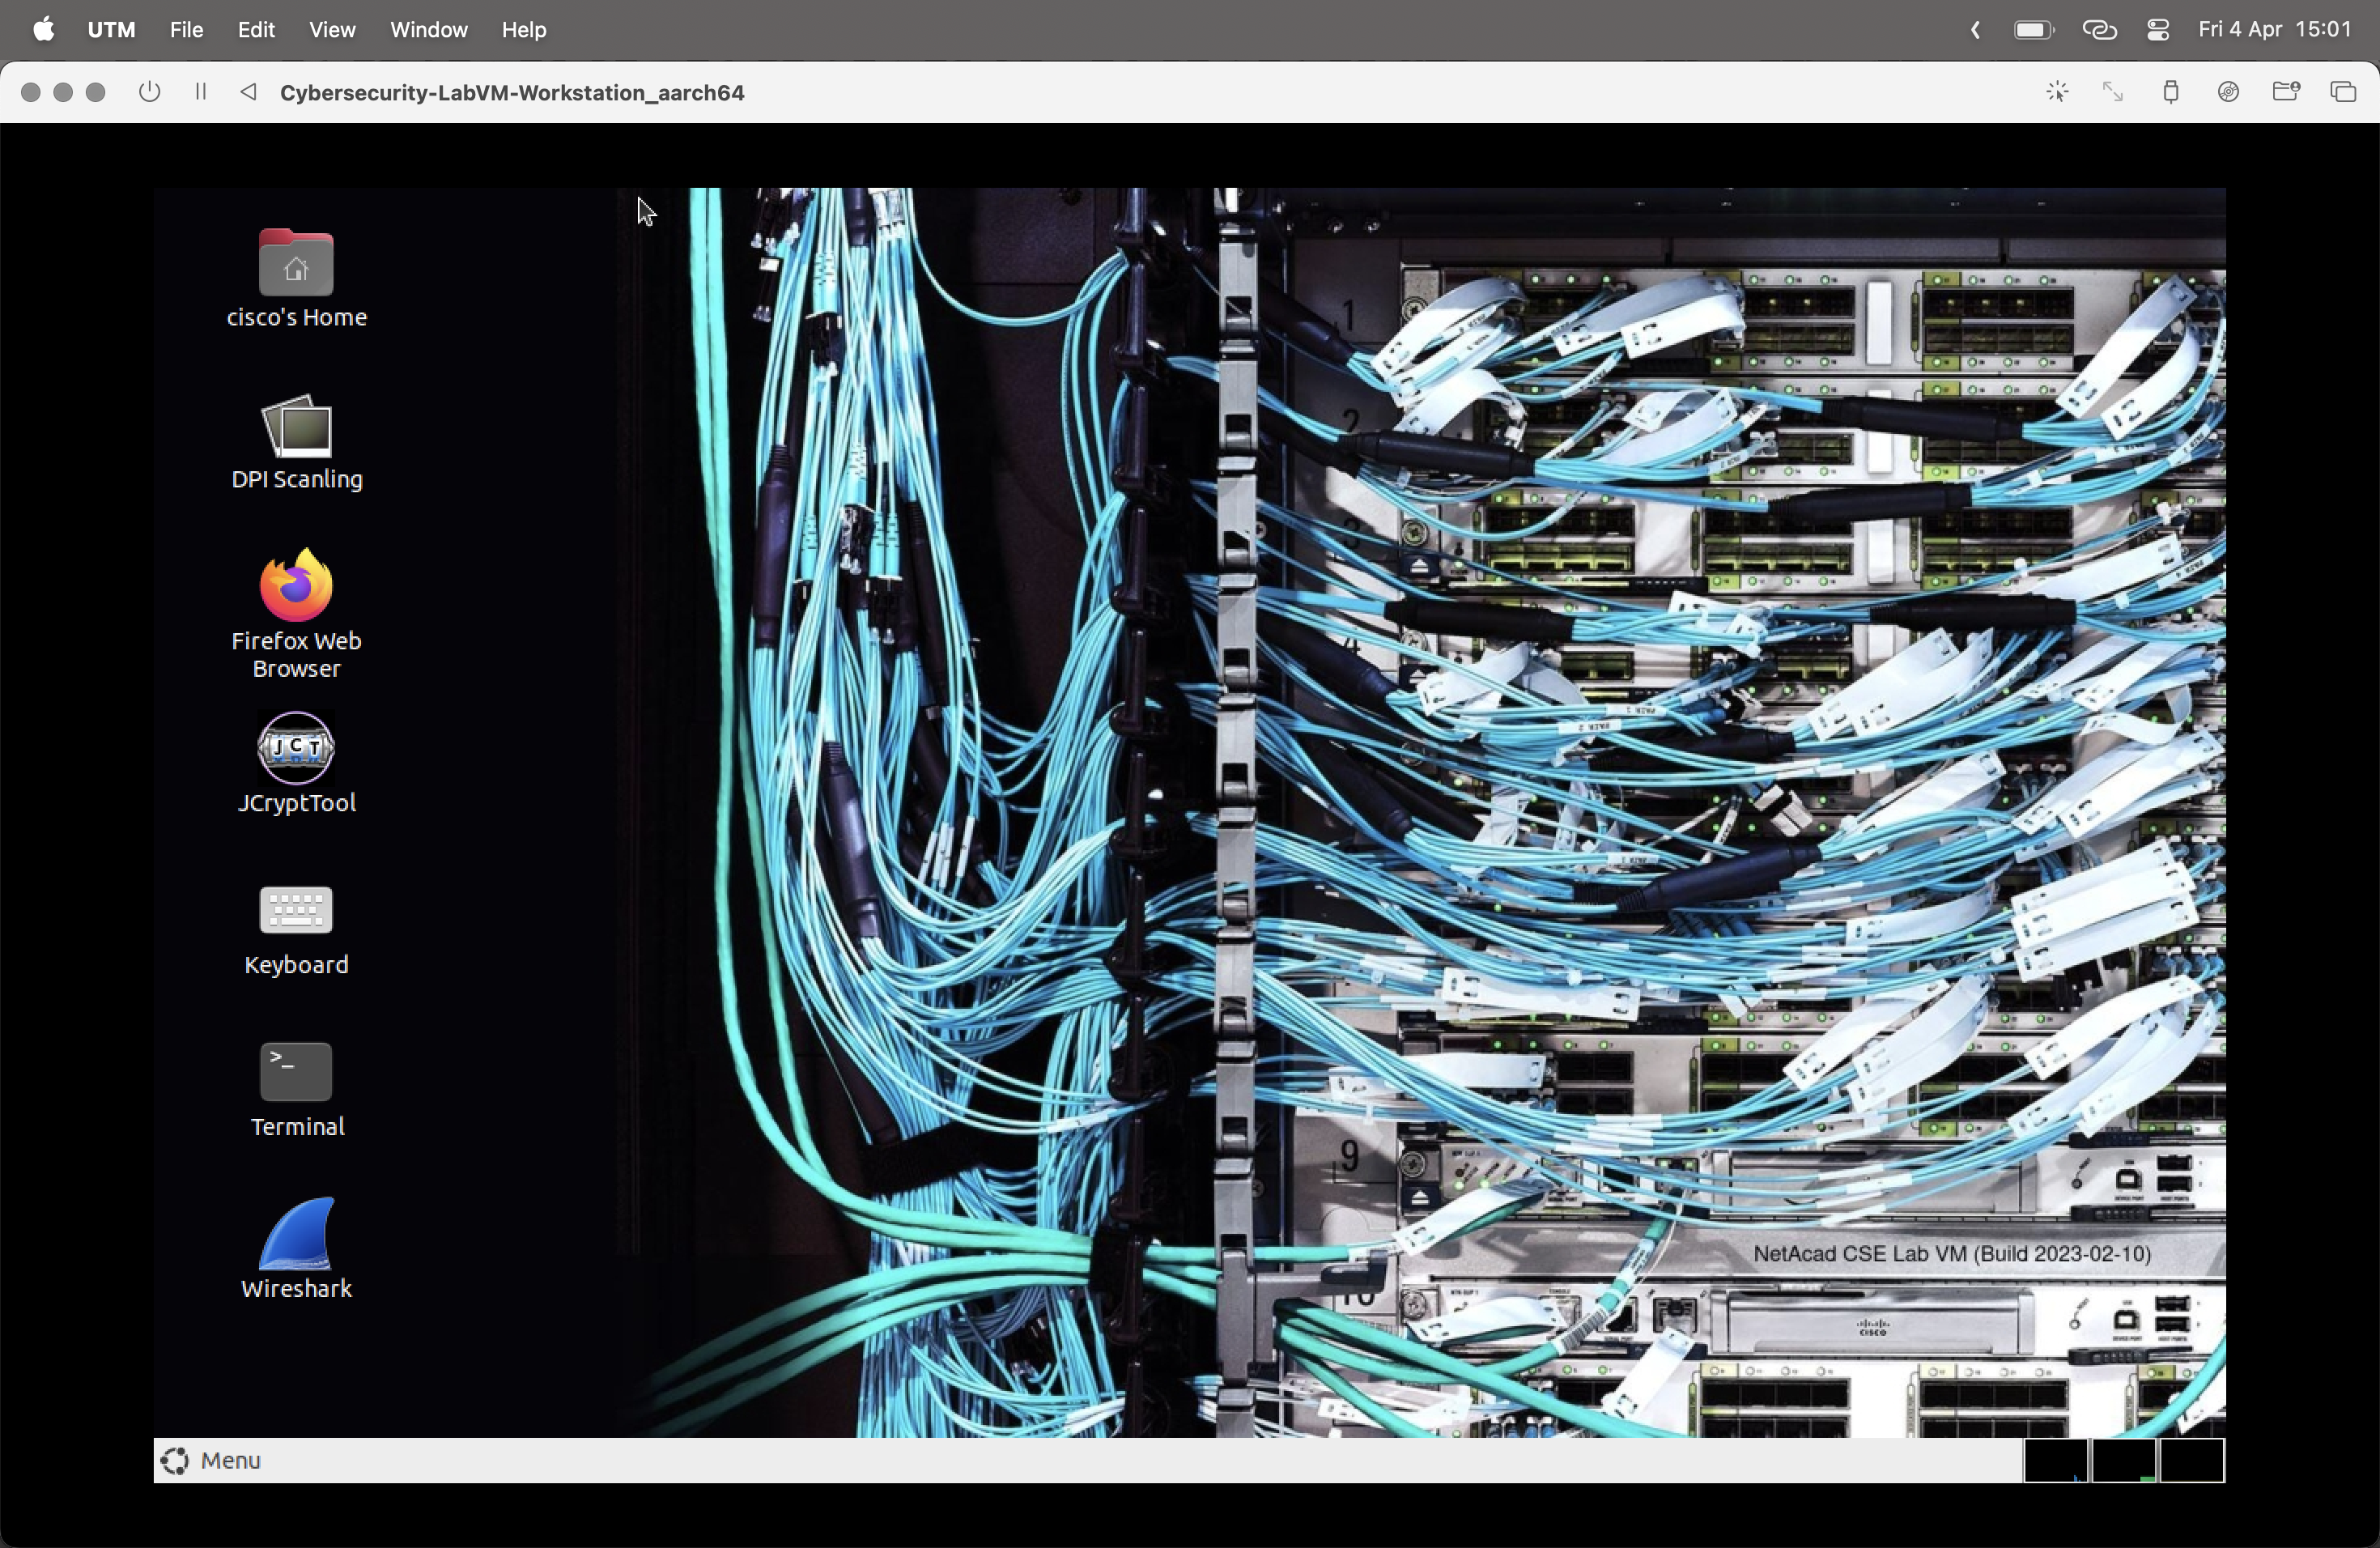
\includegraphics[width=0.8\textwidth]{lab1_vm_login.png}
    \caption{CSE-LABVM login screen}
\end{figure}

\subsubsection{Open and explore the JCrypTool}
I opened the JCrypTool application and explored its main windows and features.
\begin{figure}[H]
    \centering
    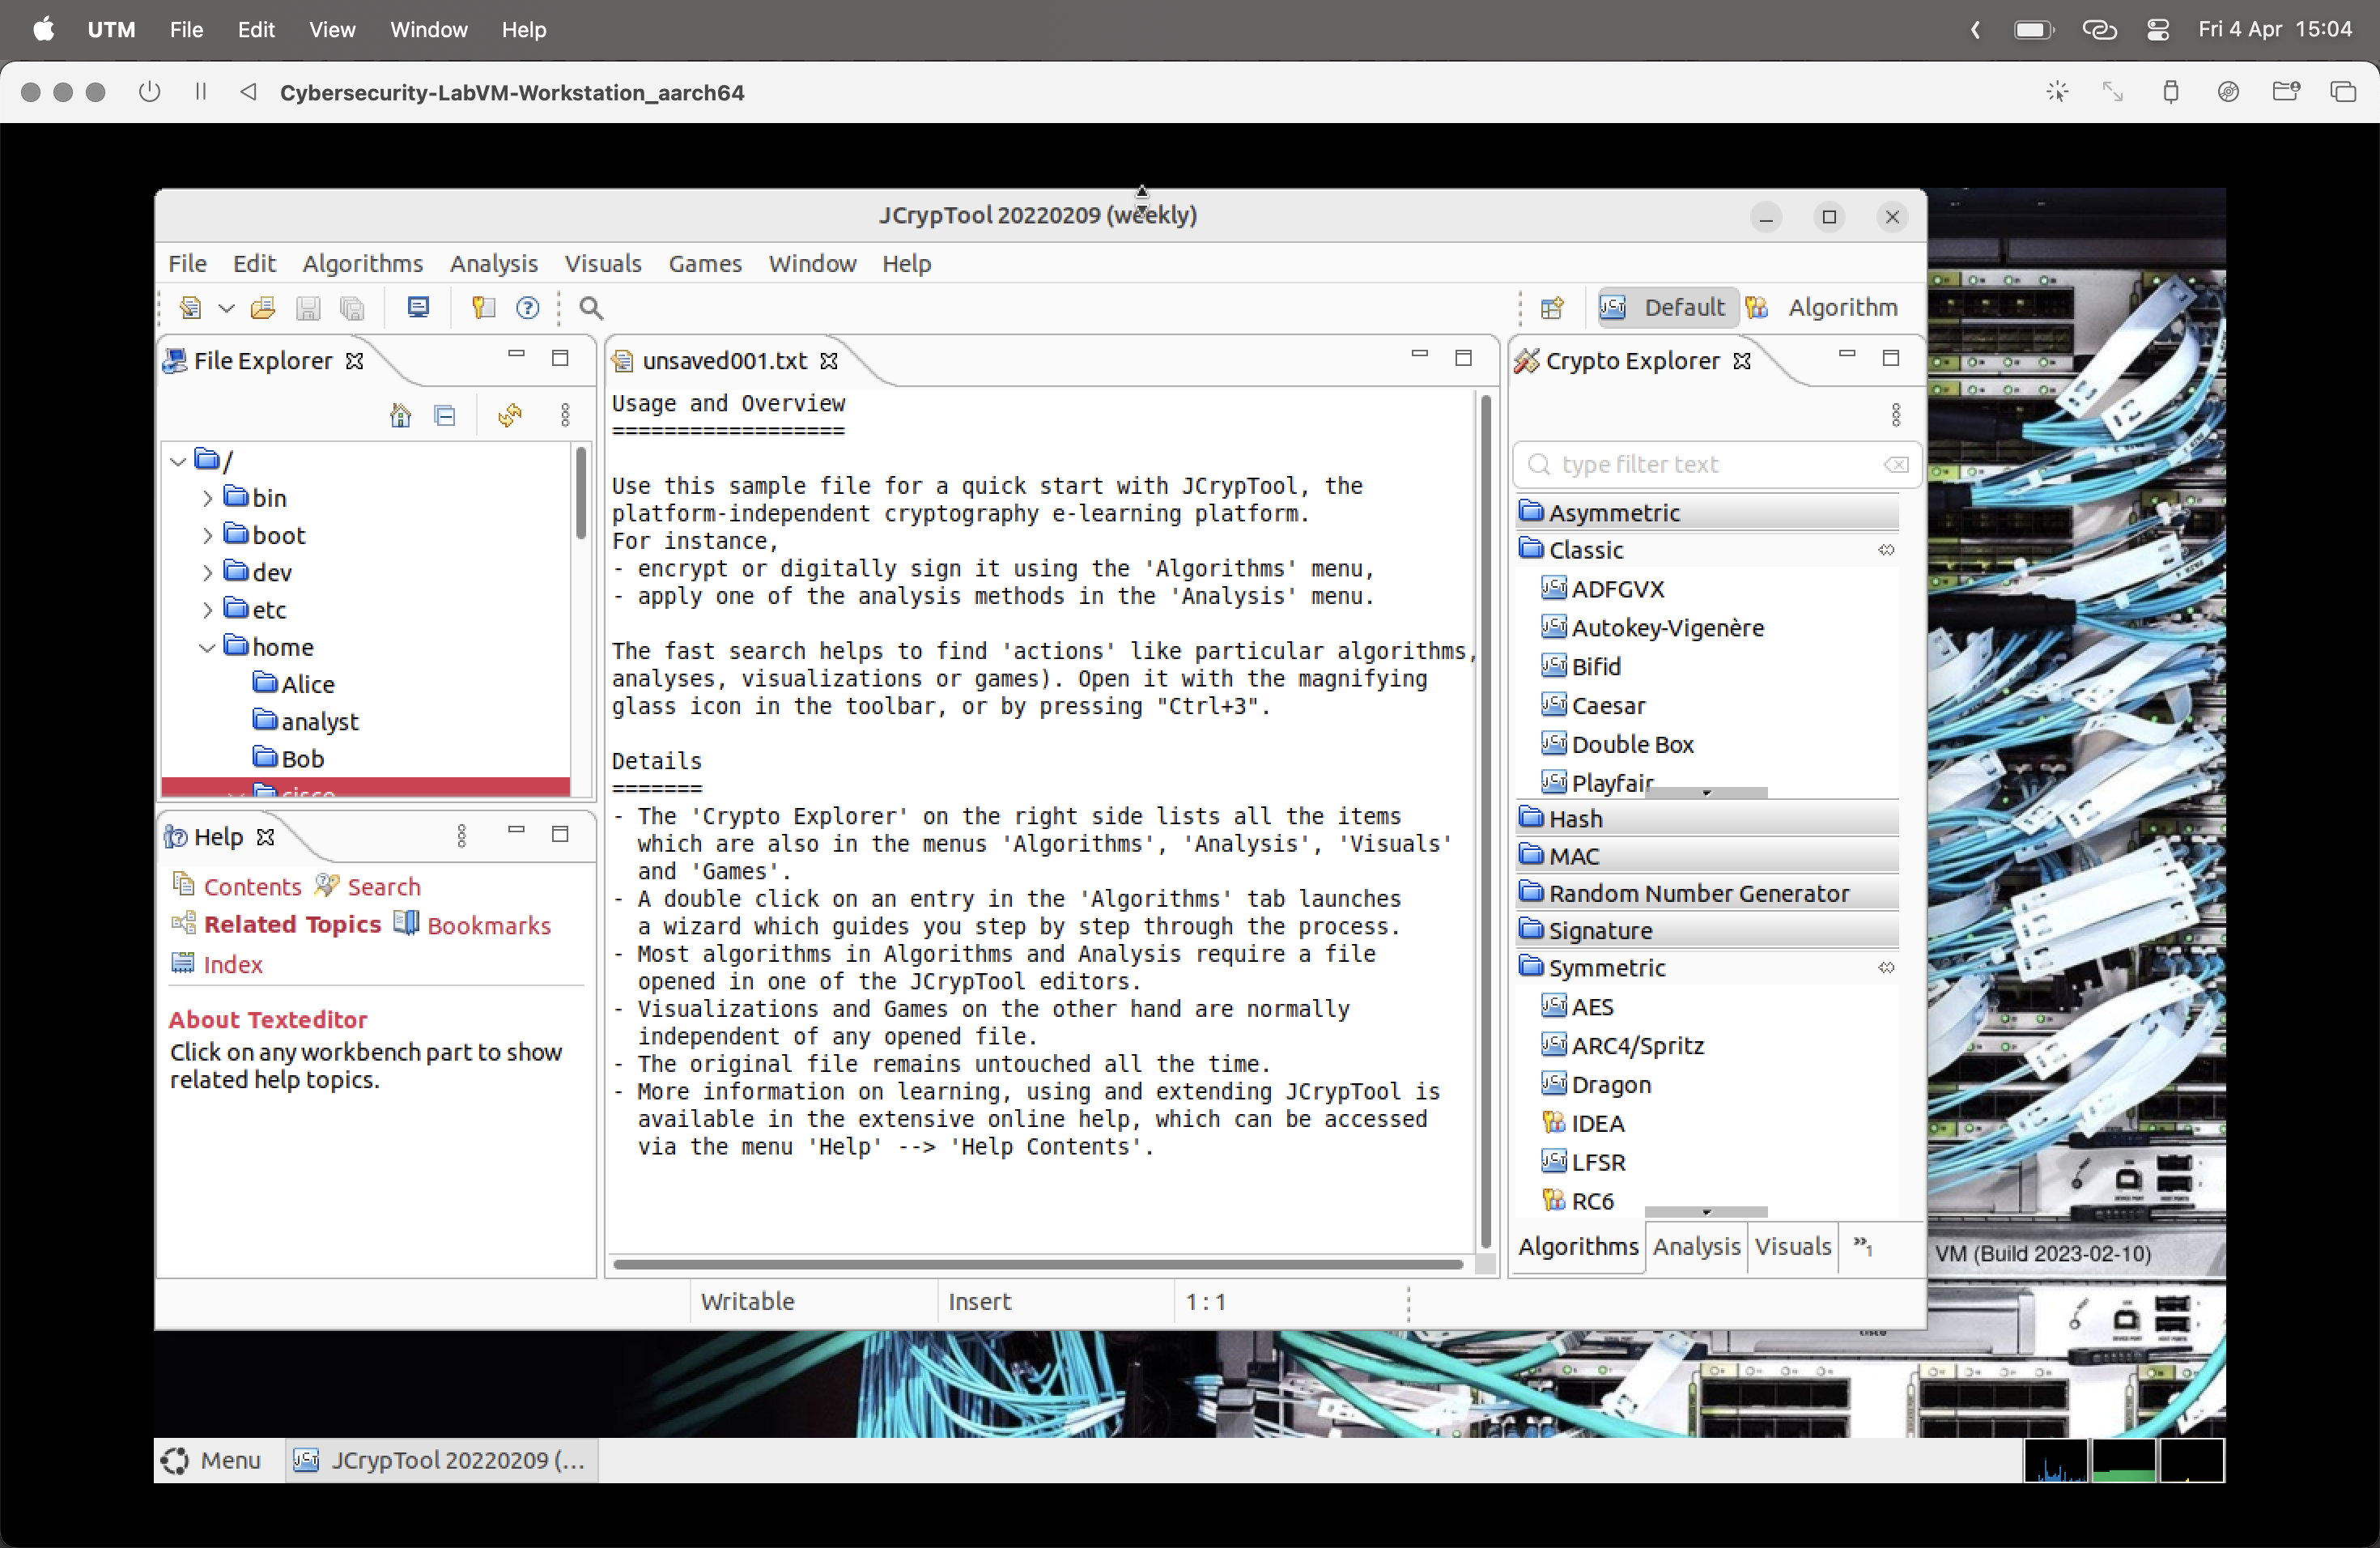
\includegraphics[width=0.8\textwidth]{lab1_JCrypTool.png}
    \caption{JCrypTool main screen}
\end{figure}

\subsubsection{Use the Caesar algorithm to encrypt a text message}
I used the Caesar algorithm to encrypt the text message "CRYPTOGRAPHY IS FUN. CAN YOU READ THIS SECRET MESSAGE?" with a JCrypTool.
\begin{figure}[H]
    \centering
    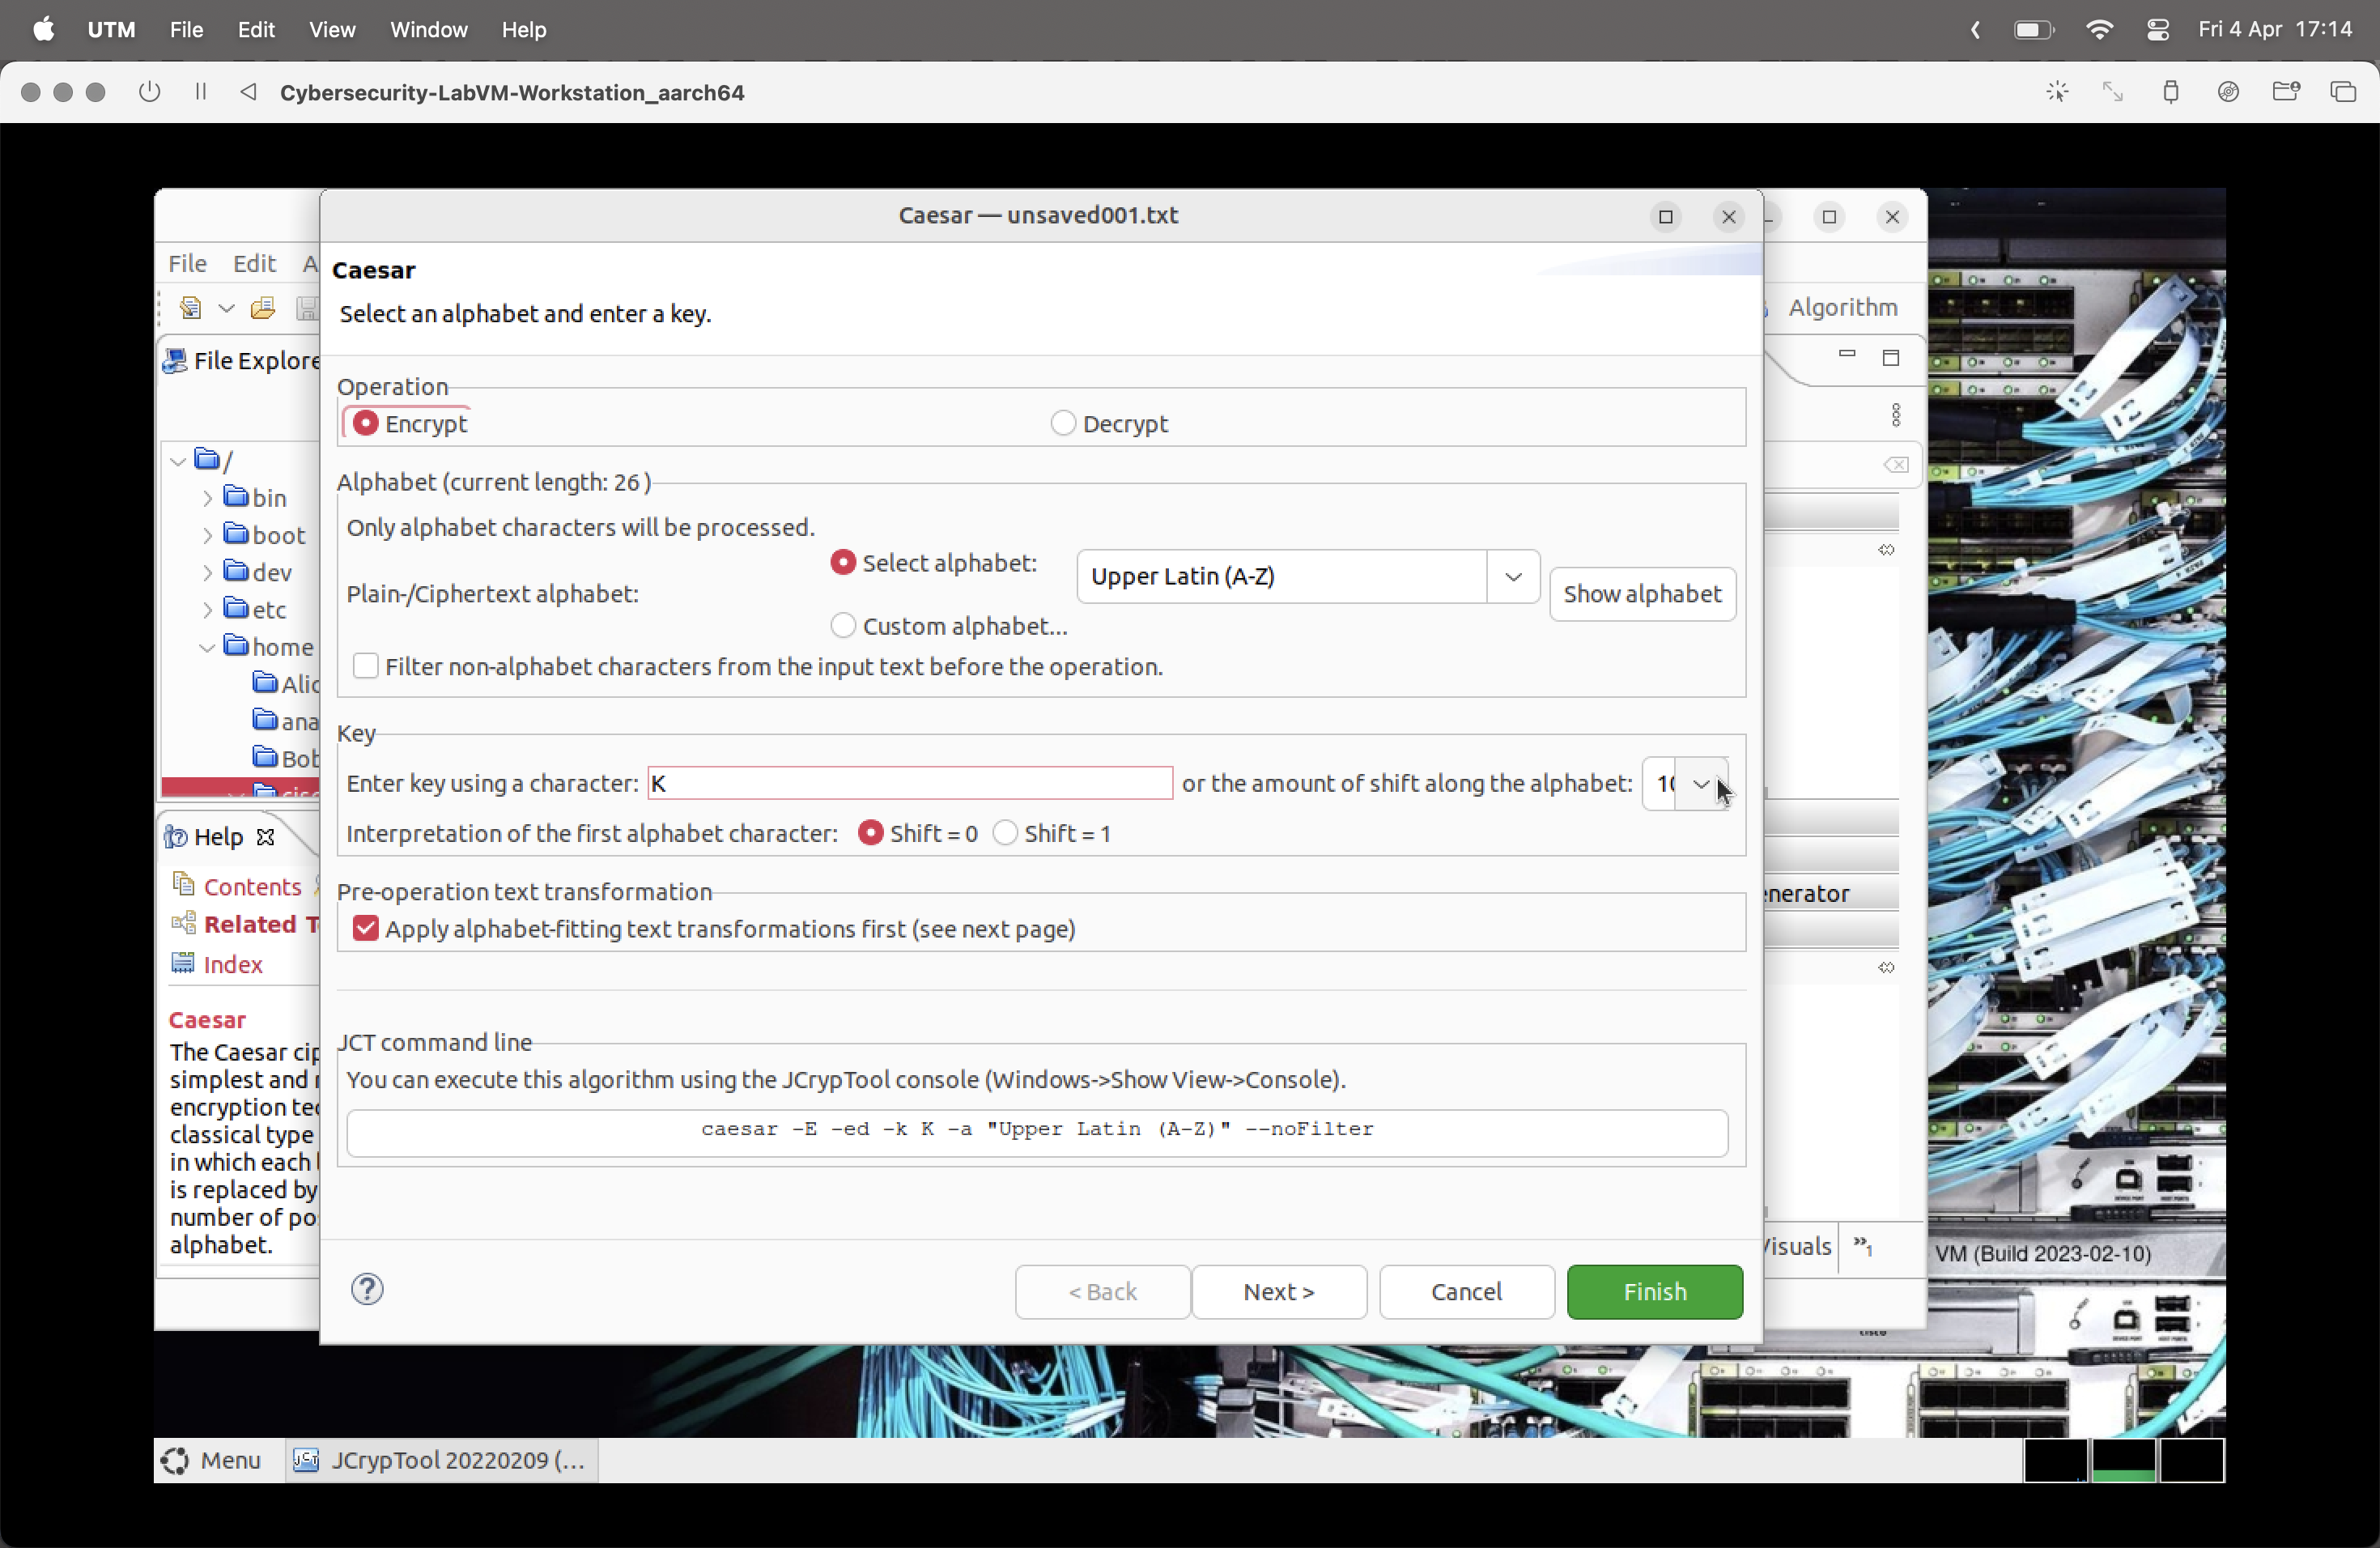
\includegraphics[width=0.8\textwidth]{lab1_JCrypTool_Caesar_configuration.png}
    \caption{JCrypTool Caesar algorithm configuration}
\end{figure}
The encrypted message was:
\texttt{MBIZDYQBKZRI SC PEX. MKX IYE BOKN DRSC COMBOD WOCCKQO?}

\newpage

\subsubsection{Decrypt the encrypted ciphertext with the Caesar algorithm.}
I decrypted the ciphertext using the same Caesar algorithm with a same configuration, but chose the "Decrypt" operation.
\begin{figure}[H]
    \centering
    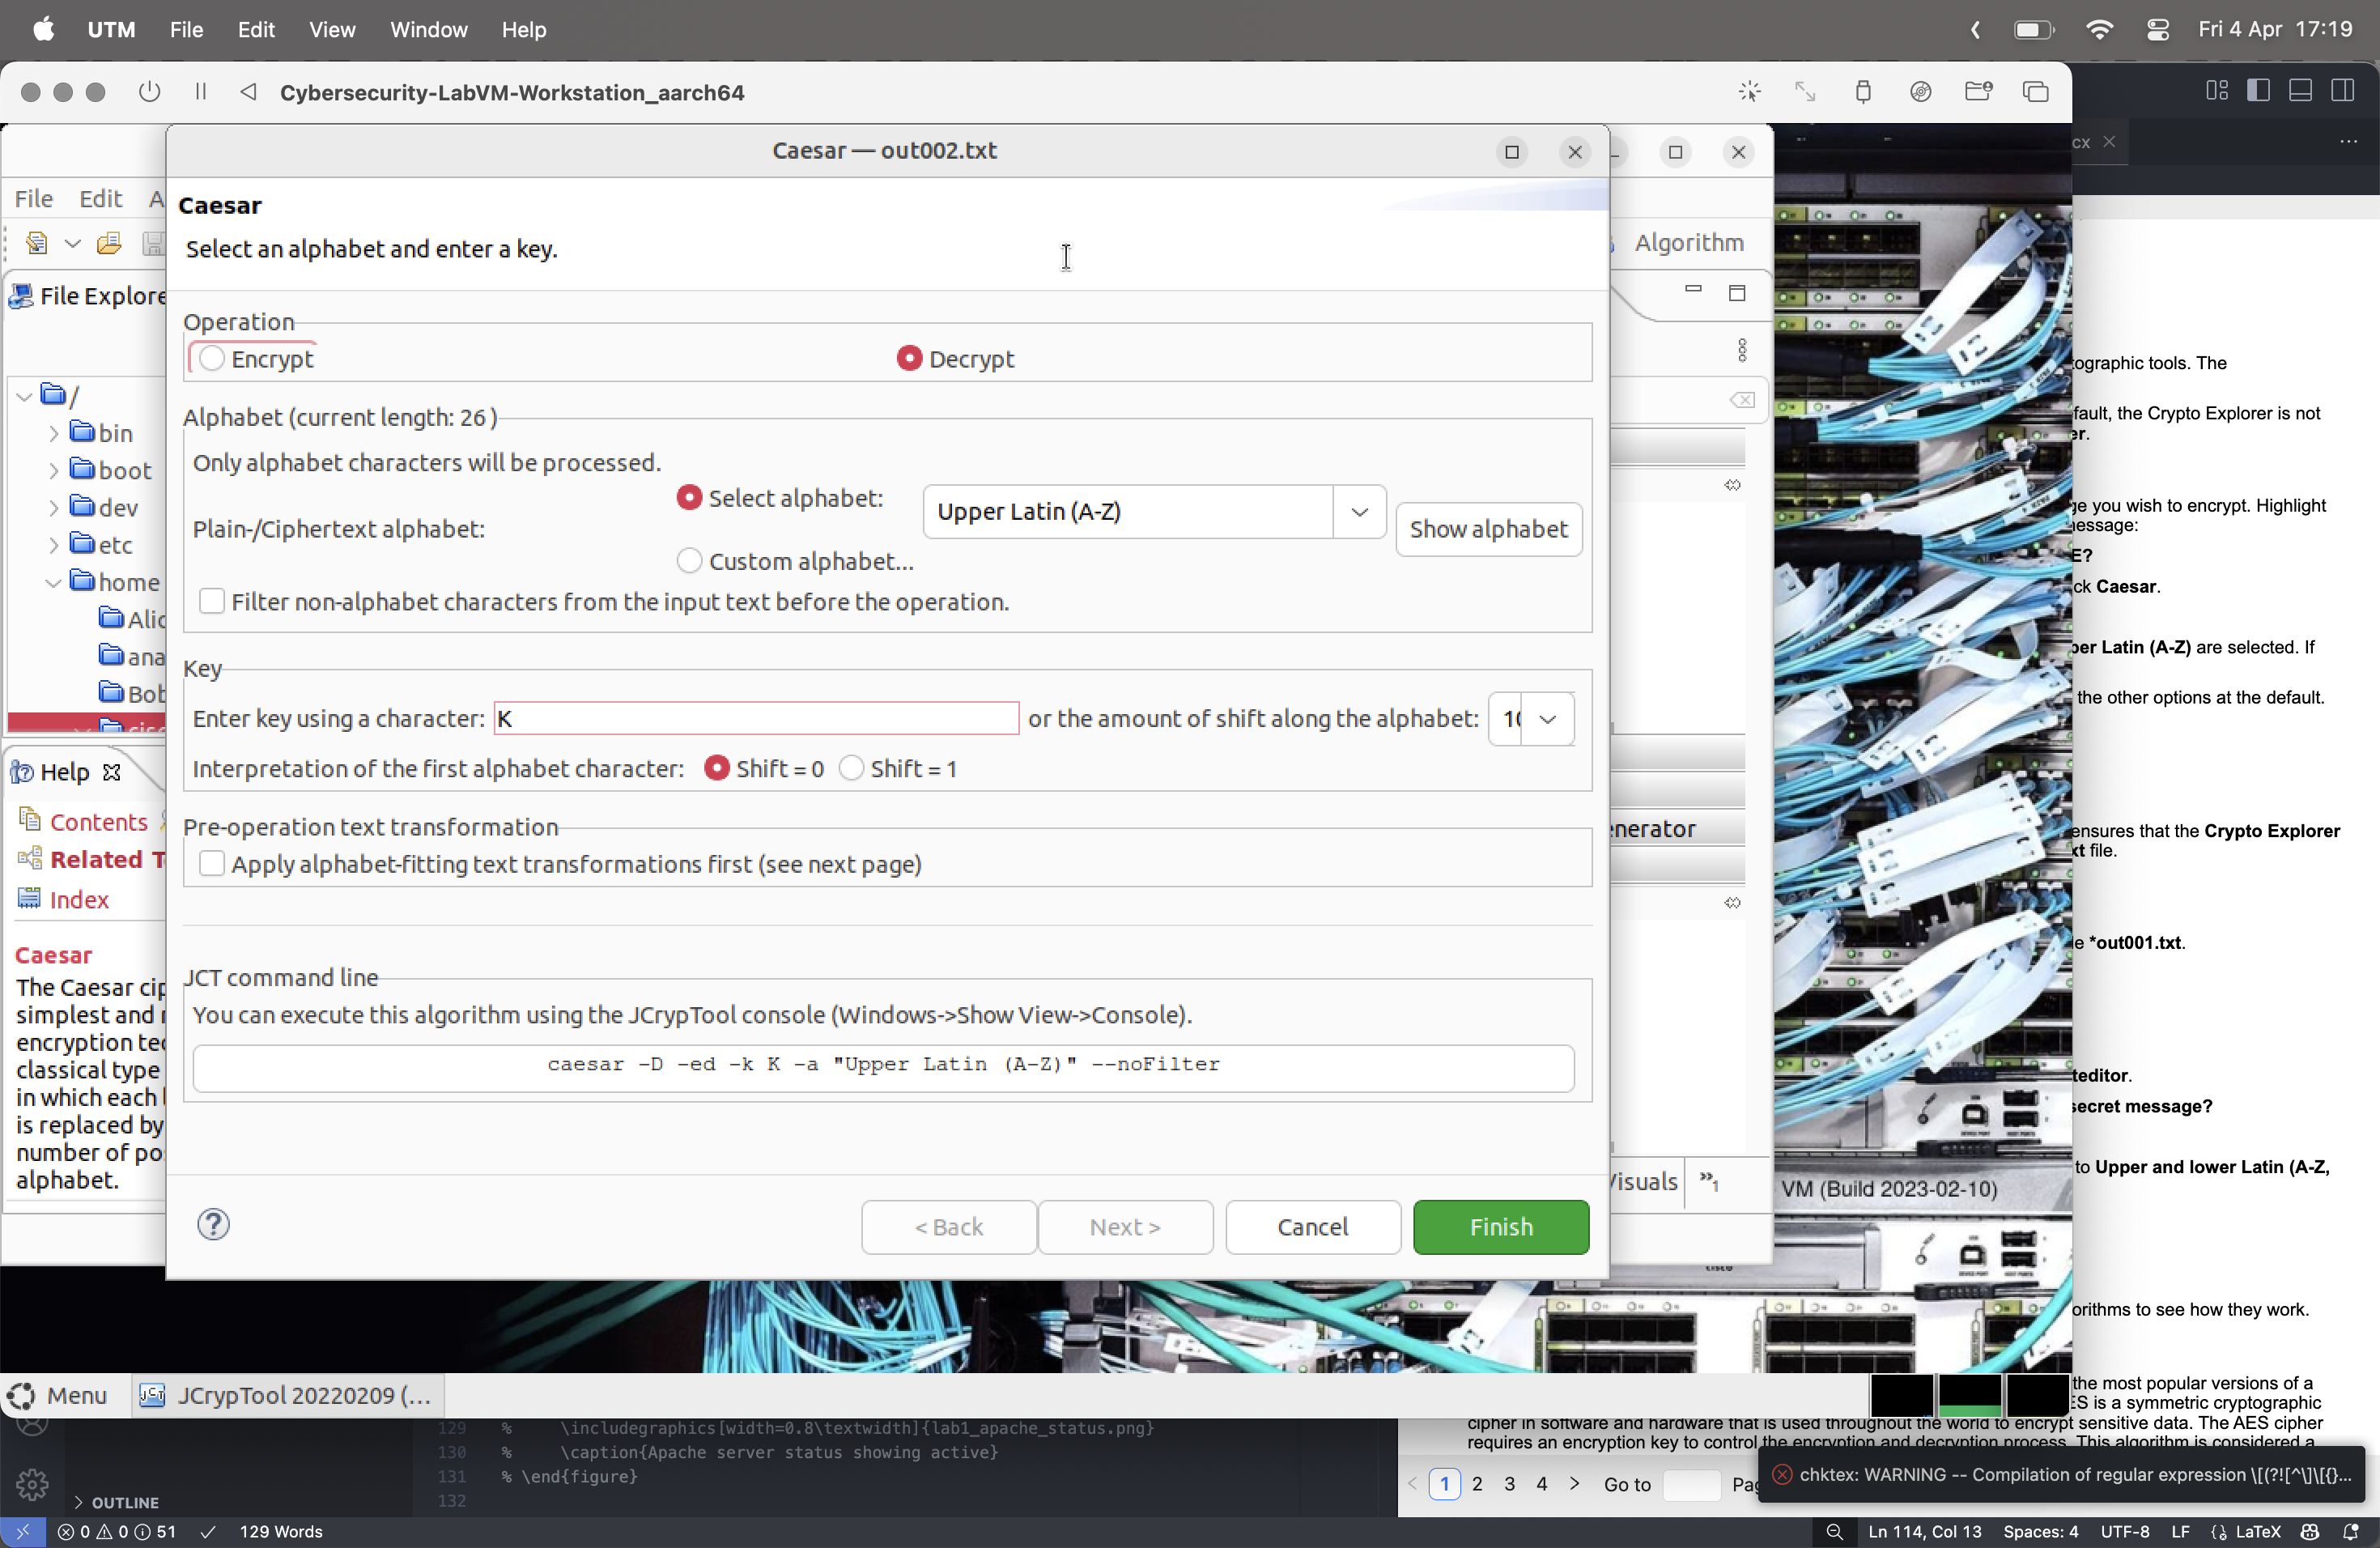
\includegraphics[width=0.8\textwidth]{lab1_JCrypTool_Caesar_configuration_decrypt.png}
    \caption{JCrypTool Caesar algorithm configuration for decryption}
\end{figure}
And yes in result I got the original message:
\texttt{CRYPTOGRAPHY IS FUN. CAN YOU READ THIS SECRET MESSAGE?}

\subsubsection{Change the Caesar algorithm settings.}
For the last step I changed the Caesar algorithm configuration and enter new message(the same but with lowercase letters):
\texttt{Cryptography is fun. Can you read this secret message?}
\begin{figure}[H]
    \centering
    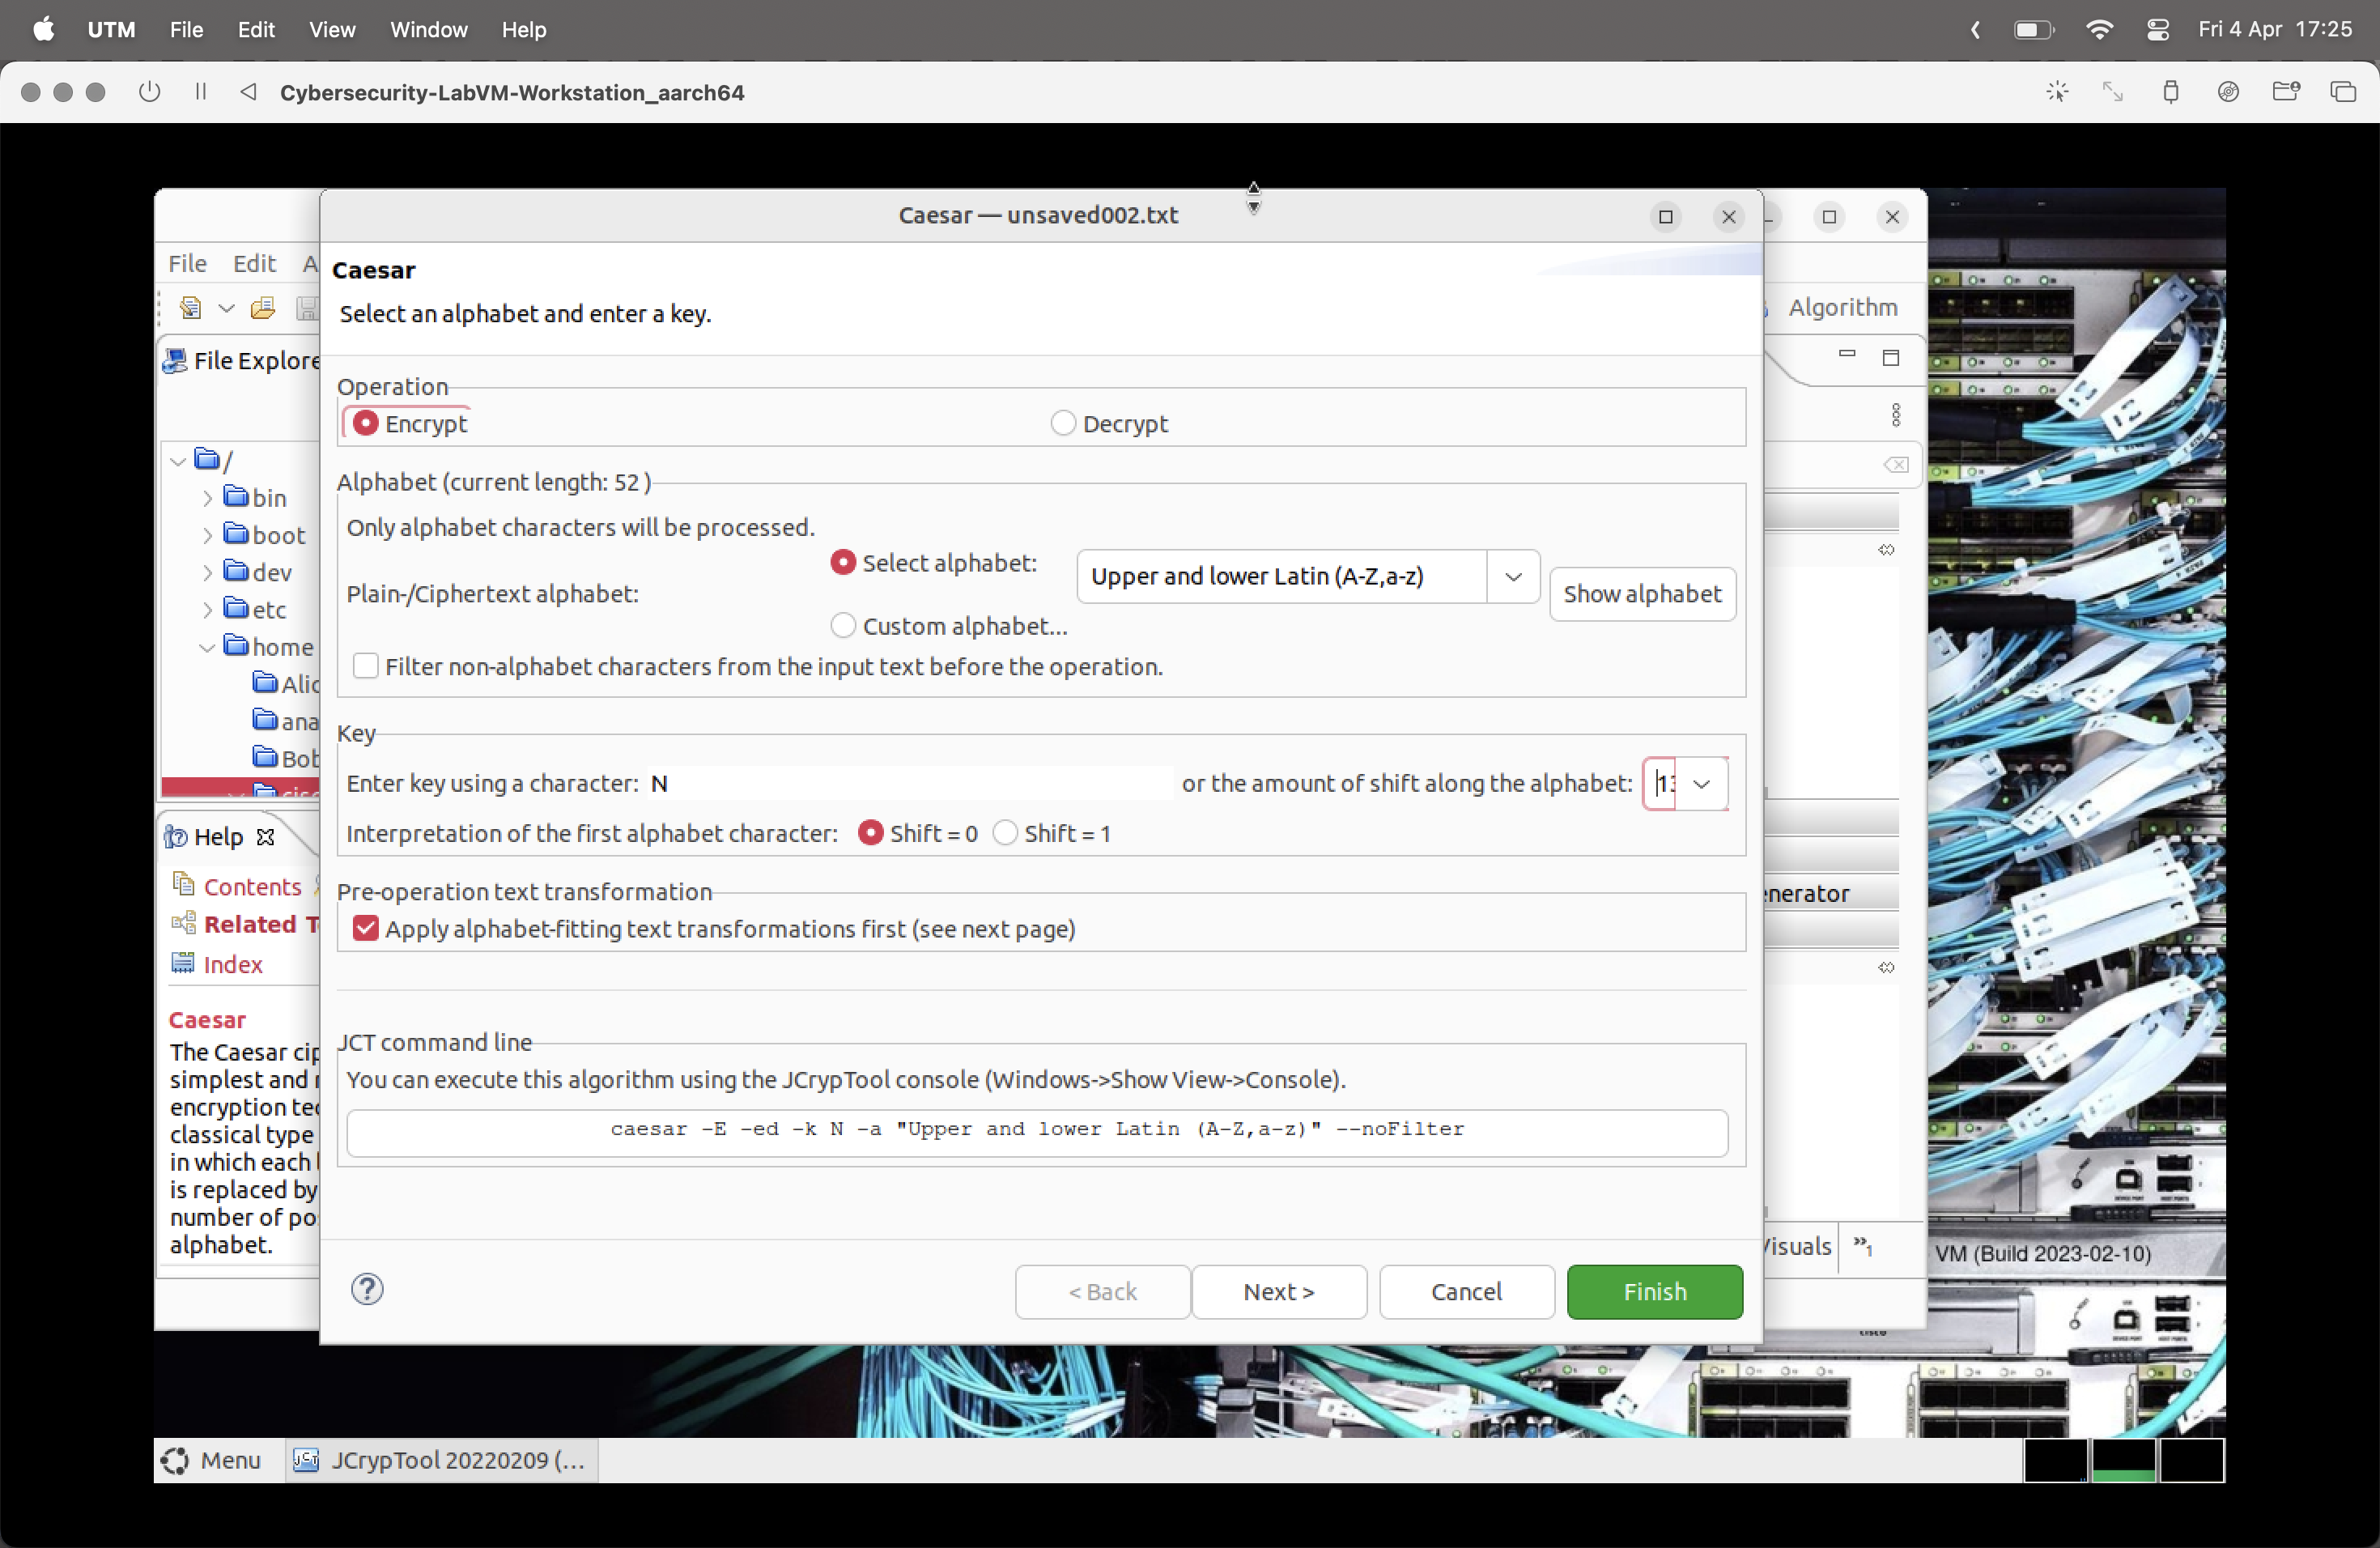
\includegraphics[width=0.8\textwidth]{lab1_JCrypTool_Caesar_changed_configuration.png}
    \caption{JCrypTool Caesar algorithm with changed configuration}
\end{figure}
The encrypted message was:
\texttt{PELCGBtEnCuL vF sHA. PnA LBH Ernq GuvF FrpErG zrFFntr?}

\subsection{Use a Modern Symmetrical Encryption Algorithm}
In this part, we will use a modern symmetrical encryption algorithm, AES(Advanced Encryption Standard).

\subsubsection{Use AES encryption to encrypt a text message.}
I used the advanced algorithm to encrypt the text message "Cryptography is fun. Can you read this secret message?" using Symmetric(AES) encryption.
\begin{figure}[H]
    \centering
    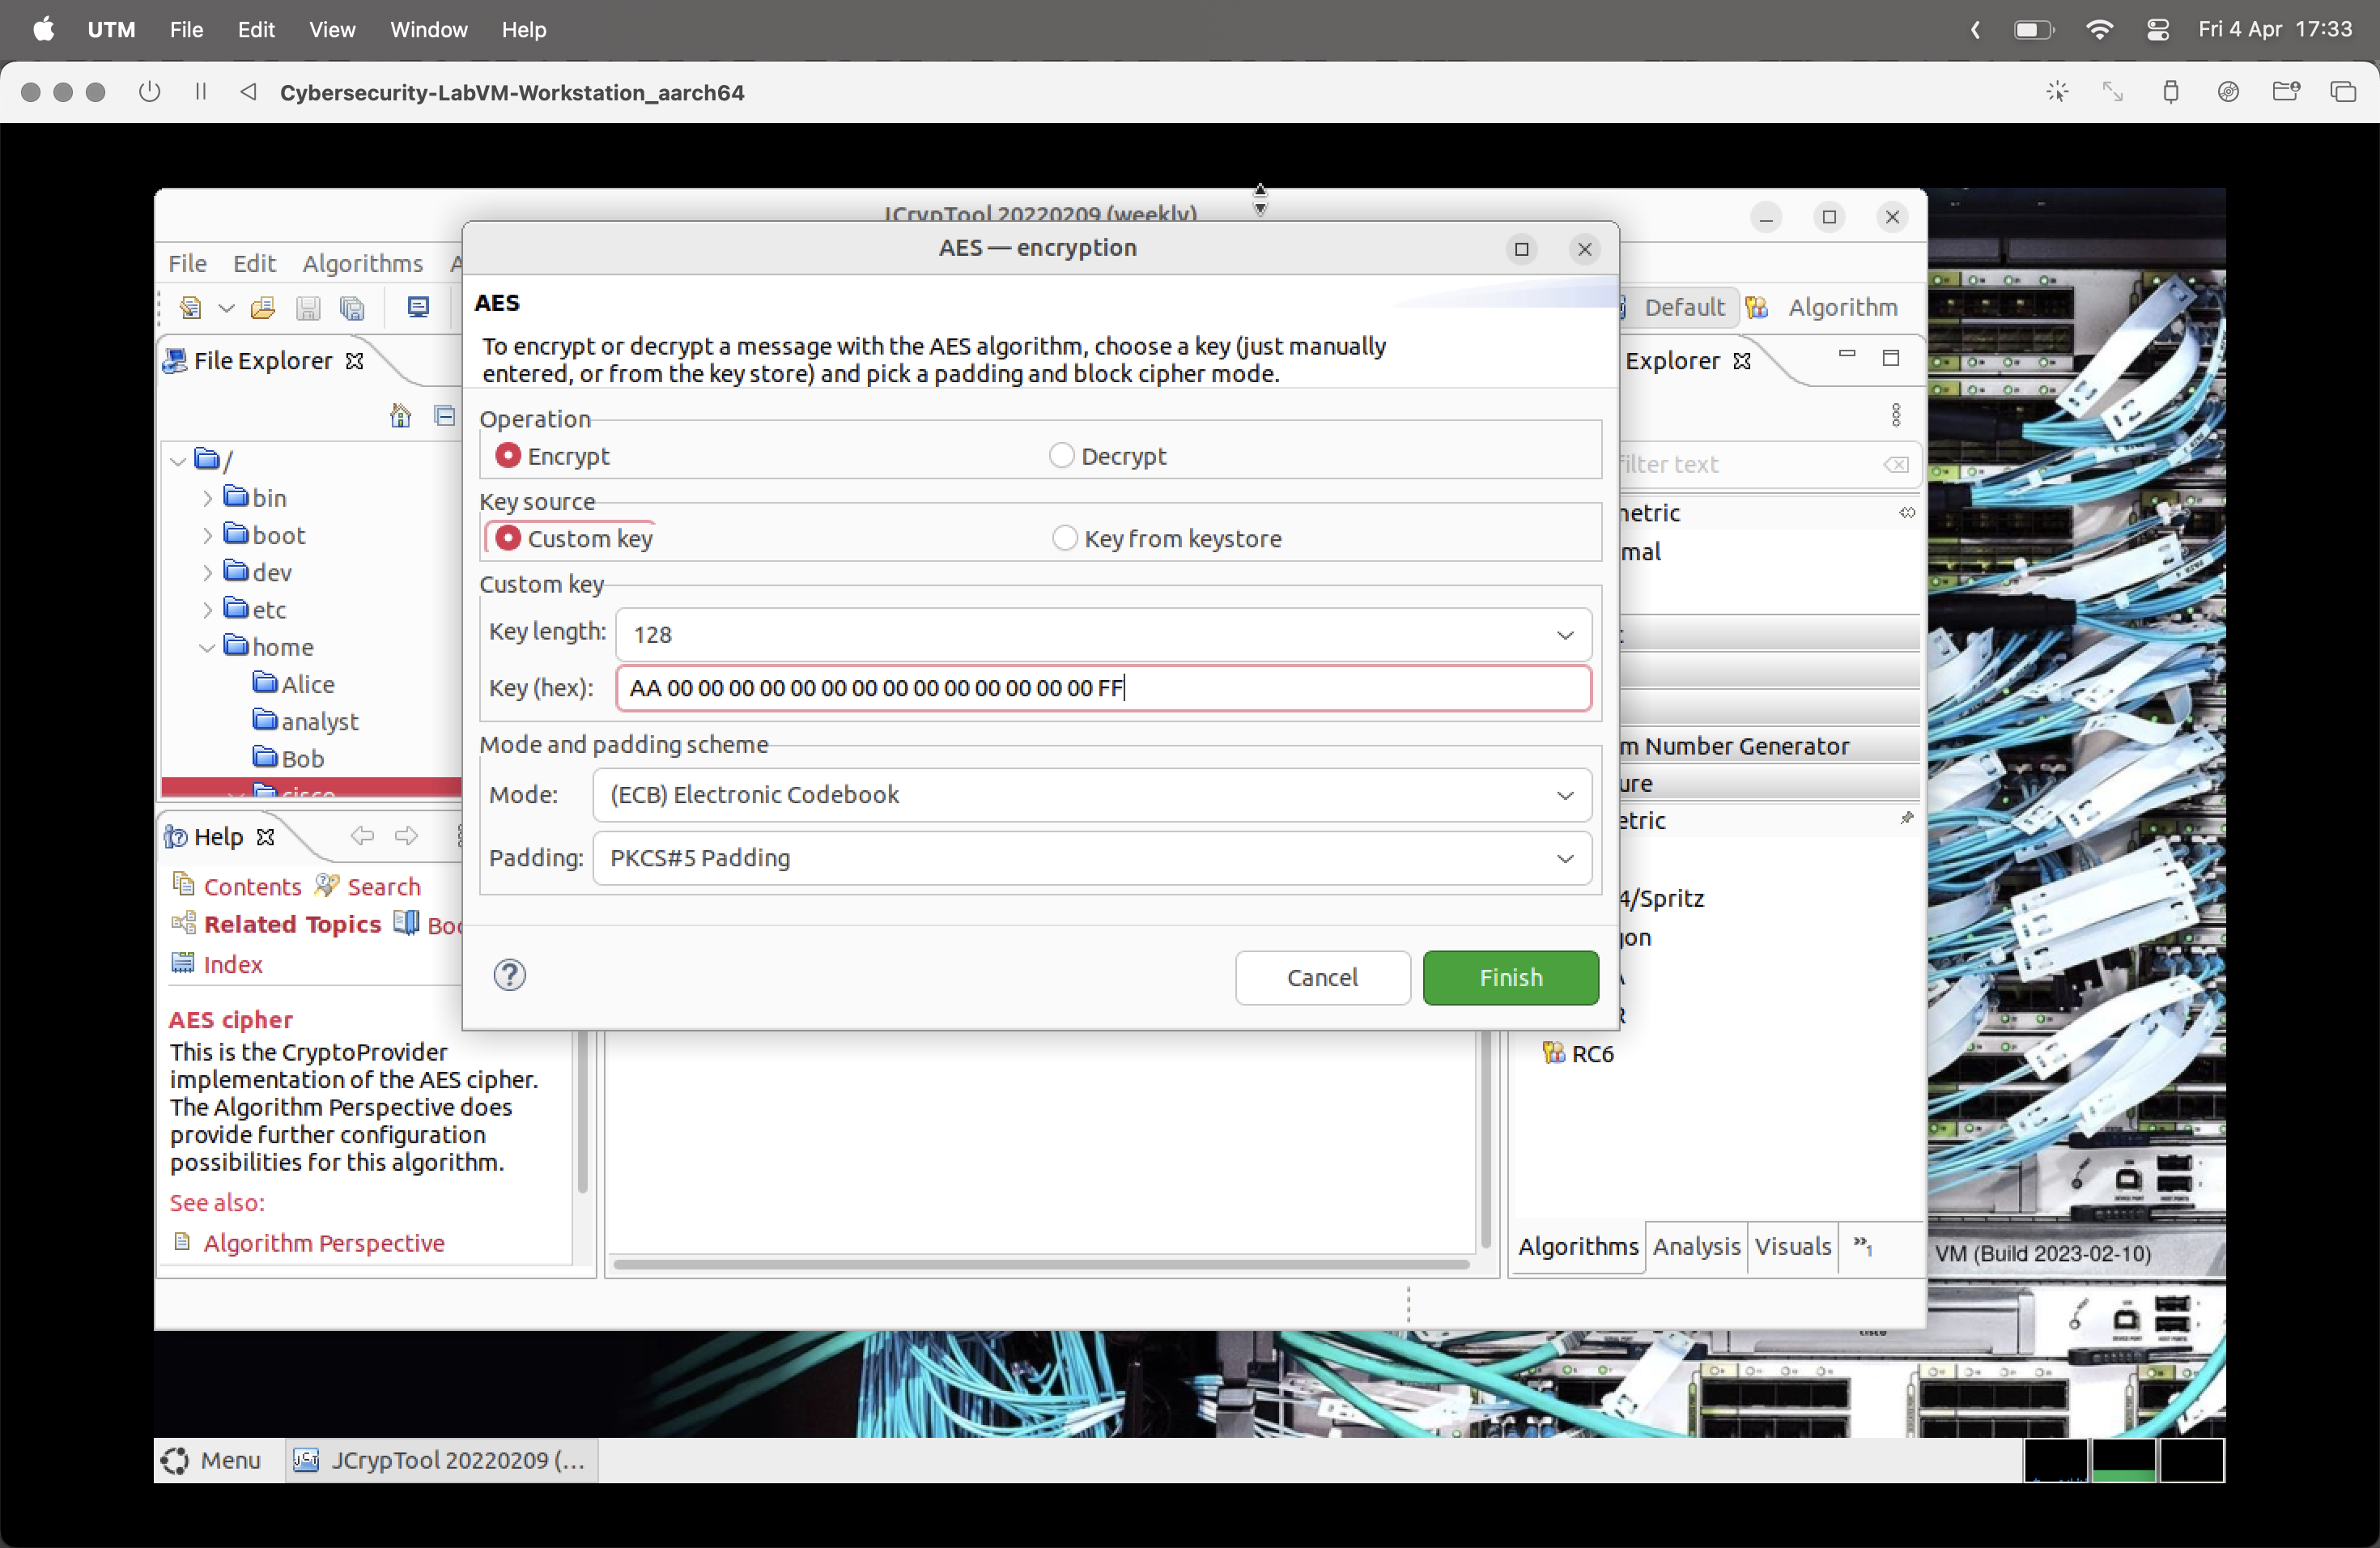
\includegraphics[width=0.8\textwidth]{lab1_JCrypTool_Symmetric_AES_config.png}
    \caption{JCrypTool Symmetric AES configuration}
\end{figure}

The encrypted message was:
\begin{figure}[H]
    \centering
    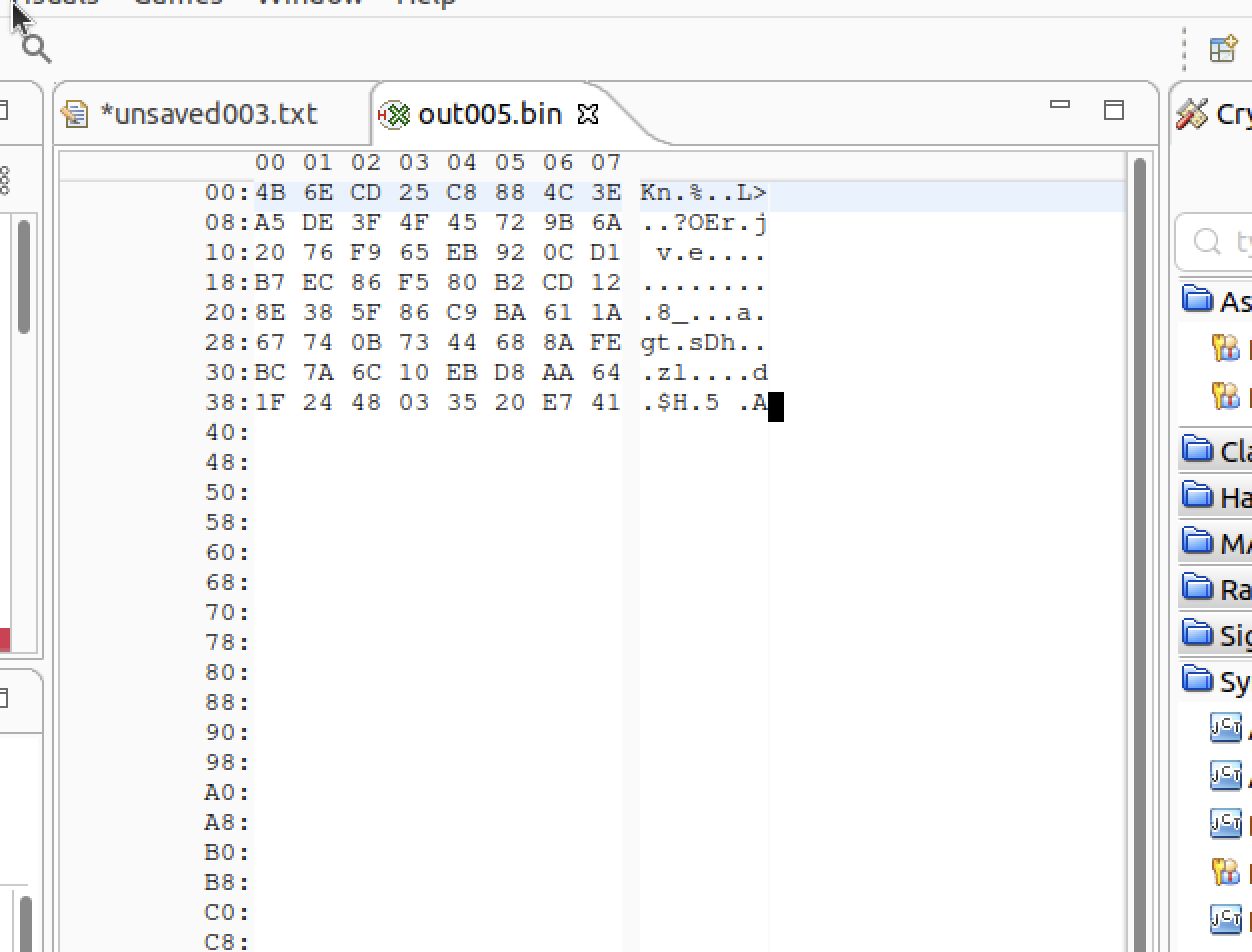
\includegraphics[width=0.8\textwidth]{lab1_JCrypTool_AES_result.png}
    \caption{JCrypTool Symmetric AES result}
\end{figure}

\subsubsection{Use AES to decrypt a text message.}
For decrypting the message. I used the same AES algorithm's configuration, but chose the "Decrypt" operation and yes for result I got the same text message encrypted.

\subsection{Use a Modern Asymmetrical Encryption Algorithm}
In this part, we will use a modern asymmetrical encryption algorithm. Unlike symmetric encryption, asymmetric encryption encrypts and decrypts the data using two separate yet mathematically connected cryptographic keys. These keys are known as a 'Public Key' and a 'Private Key'. 

\subsubsection{Use RSA asymmetrical encryption to encrypt a text file.}
There we used again the same message for encryption "Cryptography is fun. Can you read this secret message?", but with Asymmetrical(RSA) algorithm.
\begin{figure}[H]
    \centering
    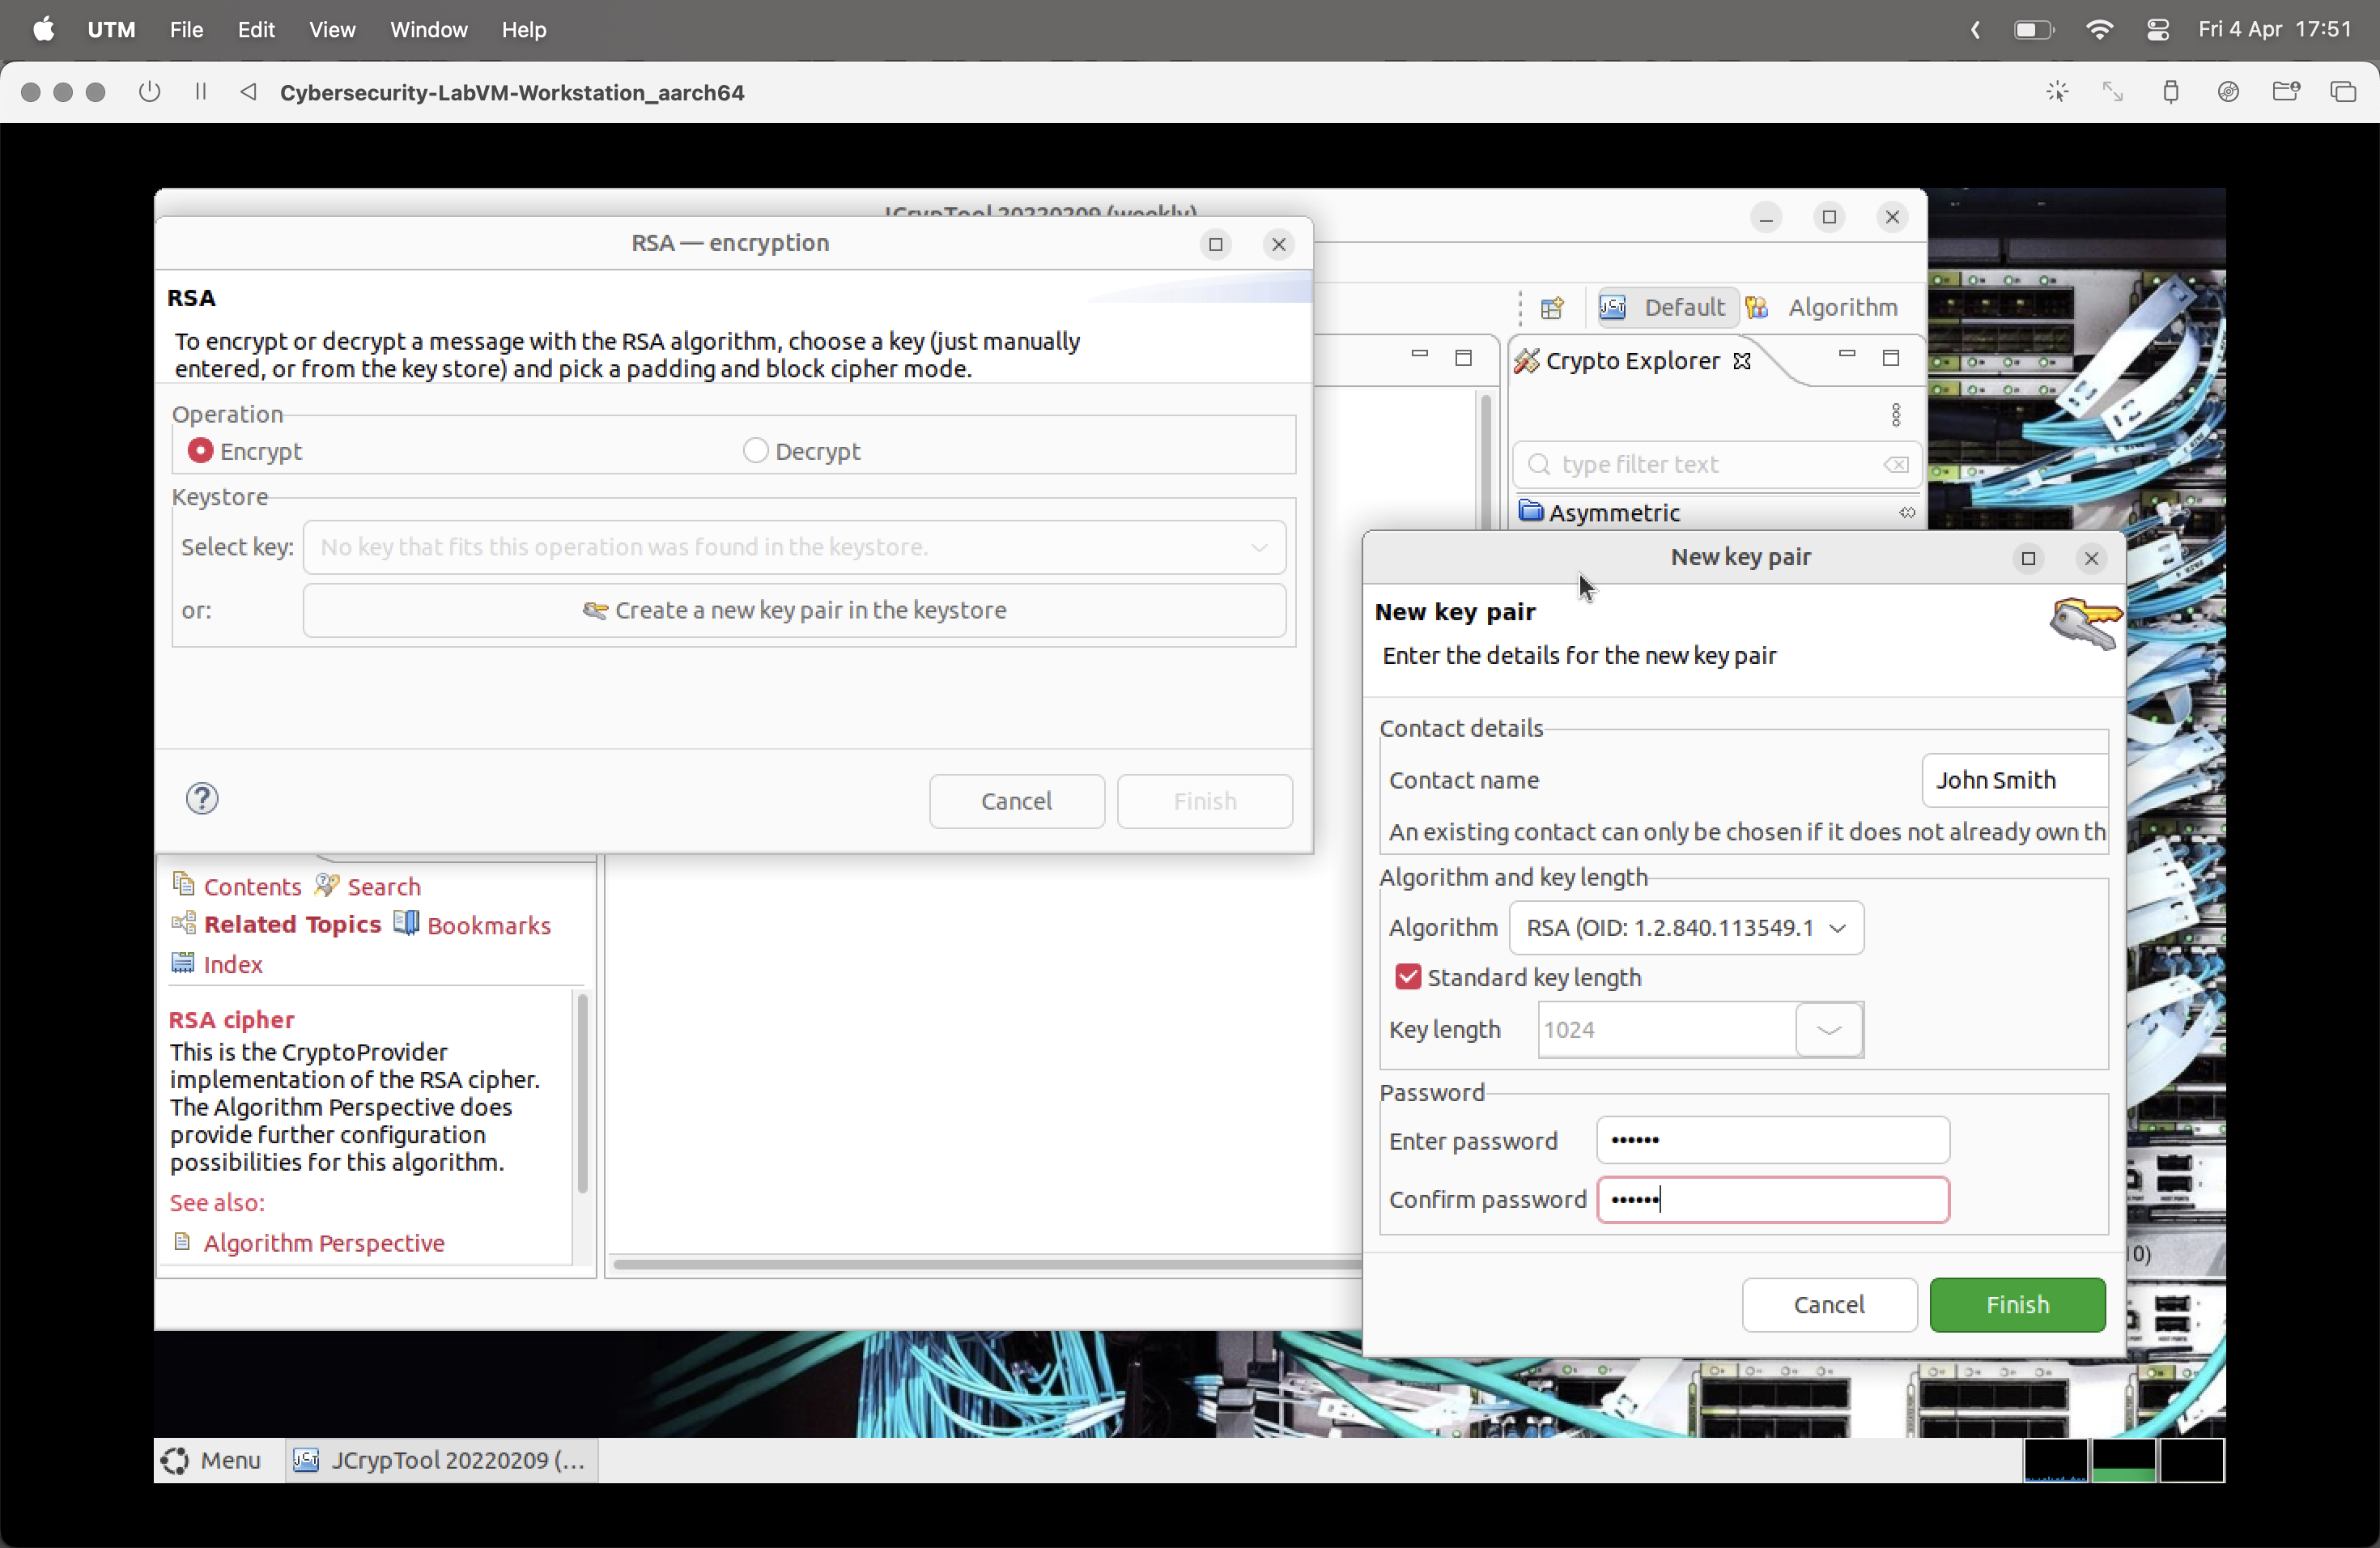
\includegraphics[width=0.8\textwidth]{lab1_JCrypTool_Asymmetric_RSA_config.png}
    \caption{JCrypTool Asymmetric RSA configuration(public/private key)}
\end{figure}

And for result I got the encrypted message:
\begin{figure}[H]
    \centering
    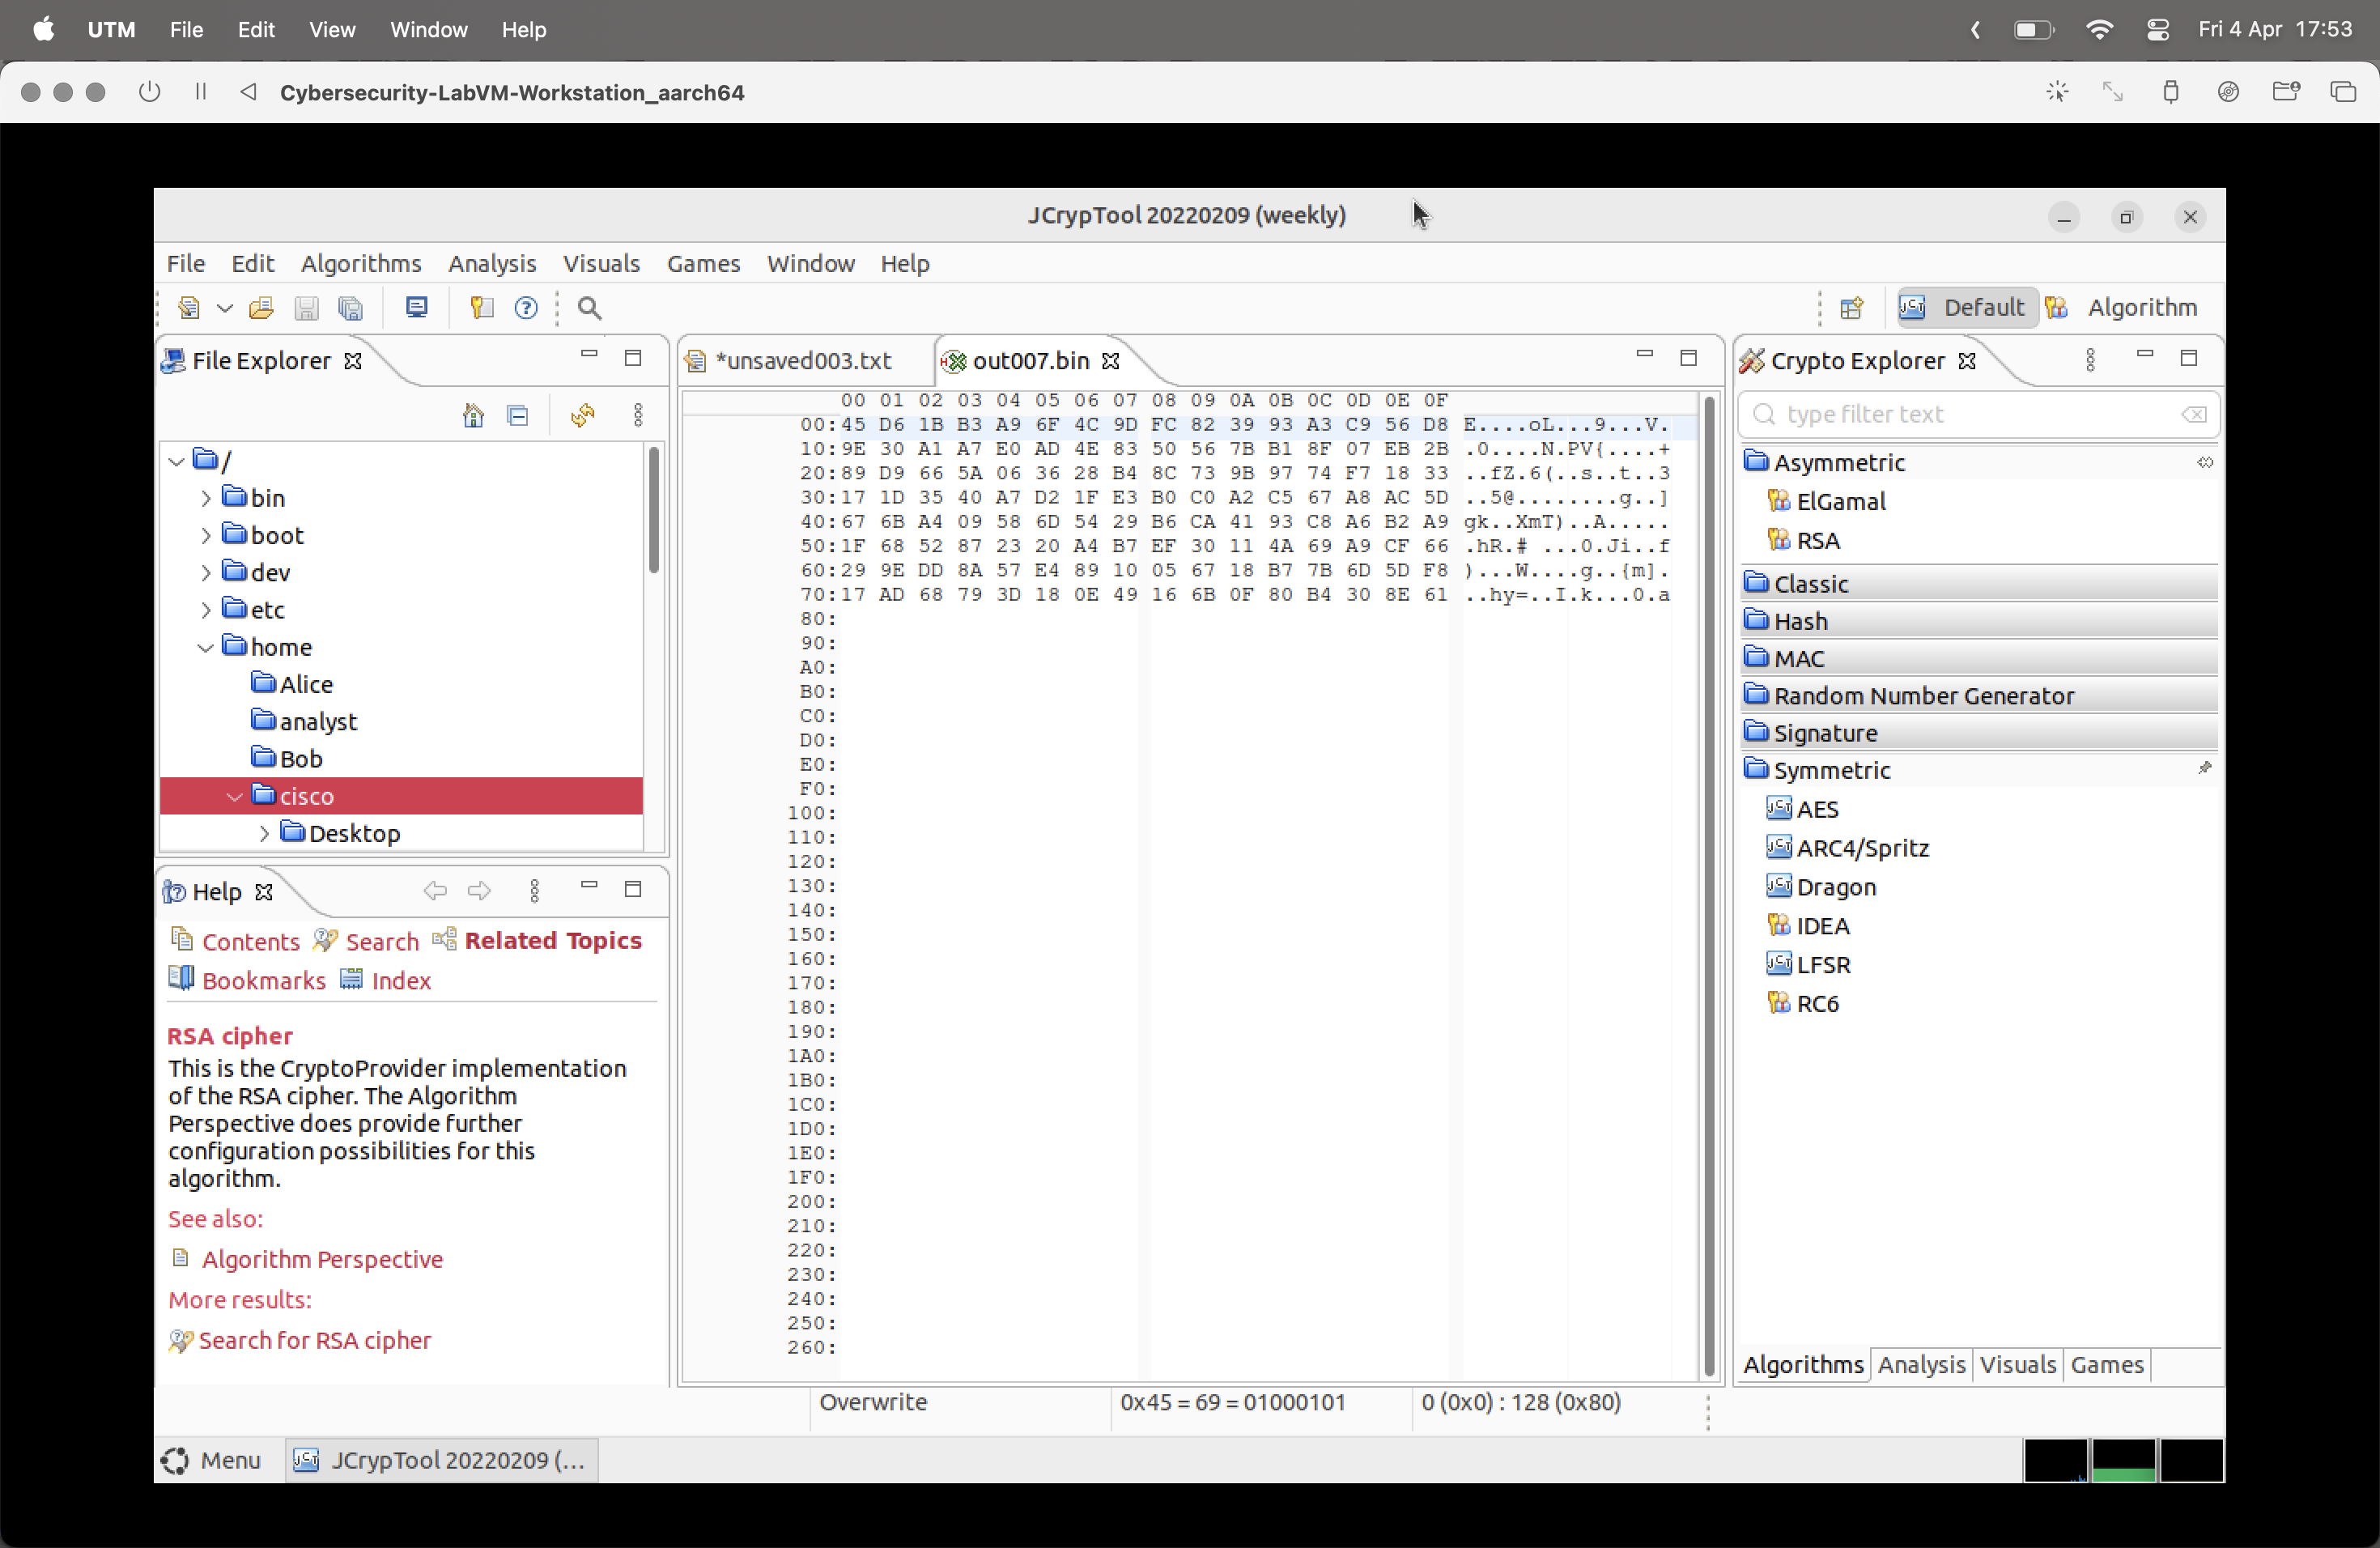
\includegraphics[width=0.8\textwidth]{lab1_JCrypTool_Asymmetric_RSA_result.png}
    \caption{JCrypTool Asymmetric RSA result}
\end{figure}

\subsubsection{Use RSA asymmetrical encryption to decrypt a text file.}
I used the private key to decrypt the encrypted message. I used the same key that was generated during the encryption process.
\begin{figure}[H]
    \centering
    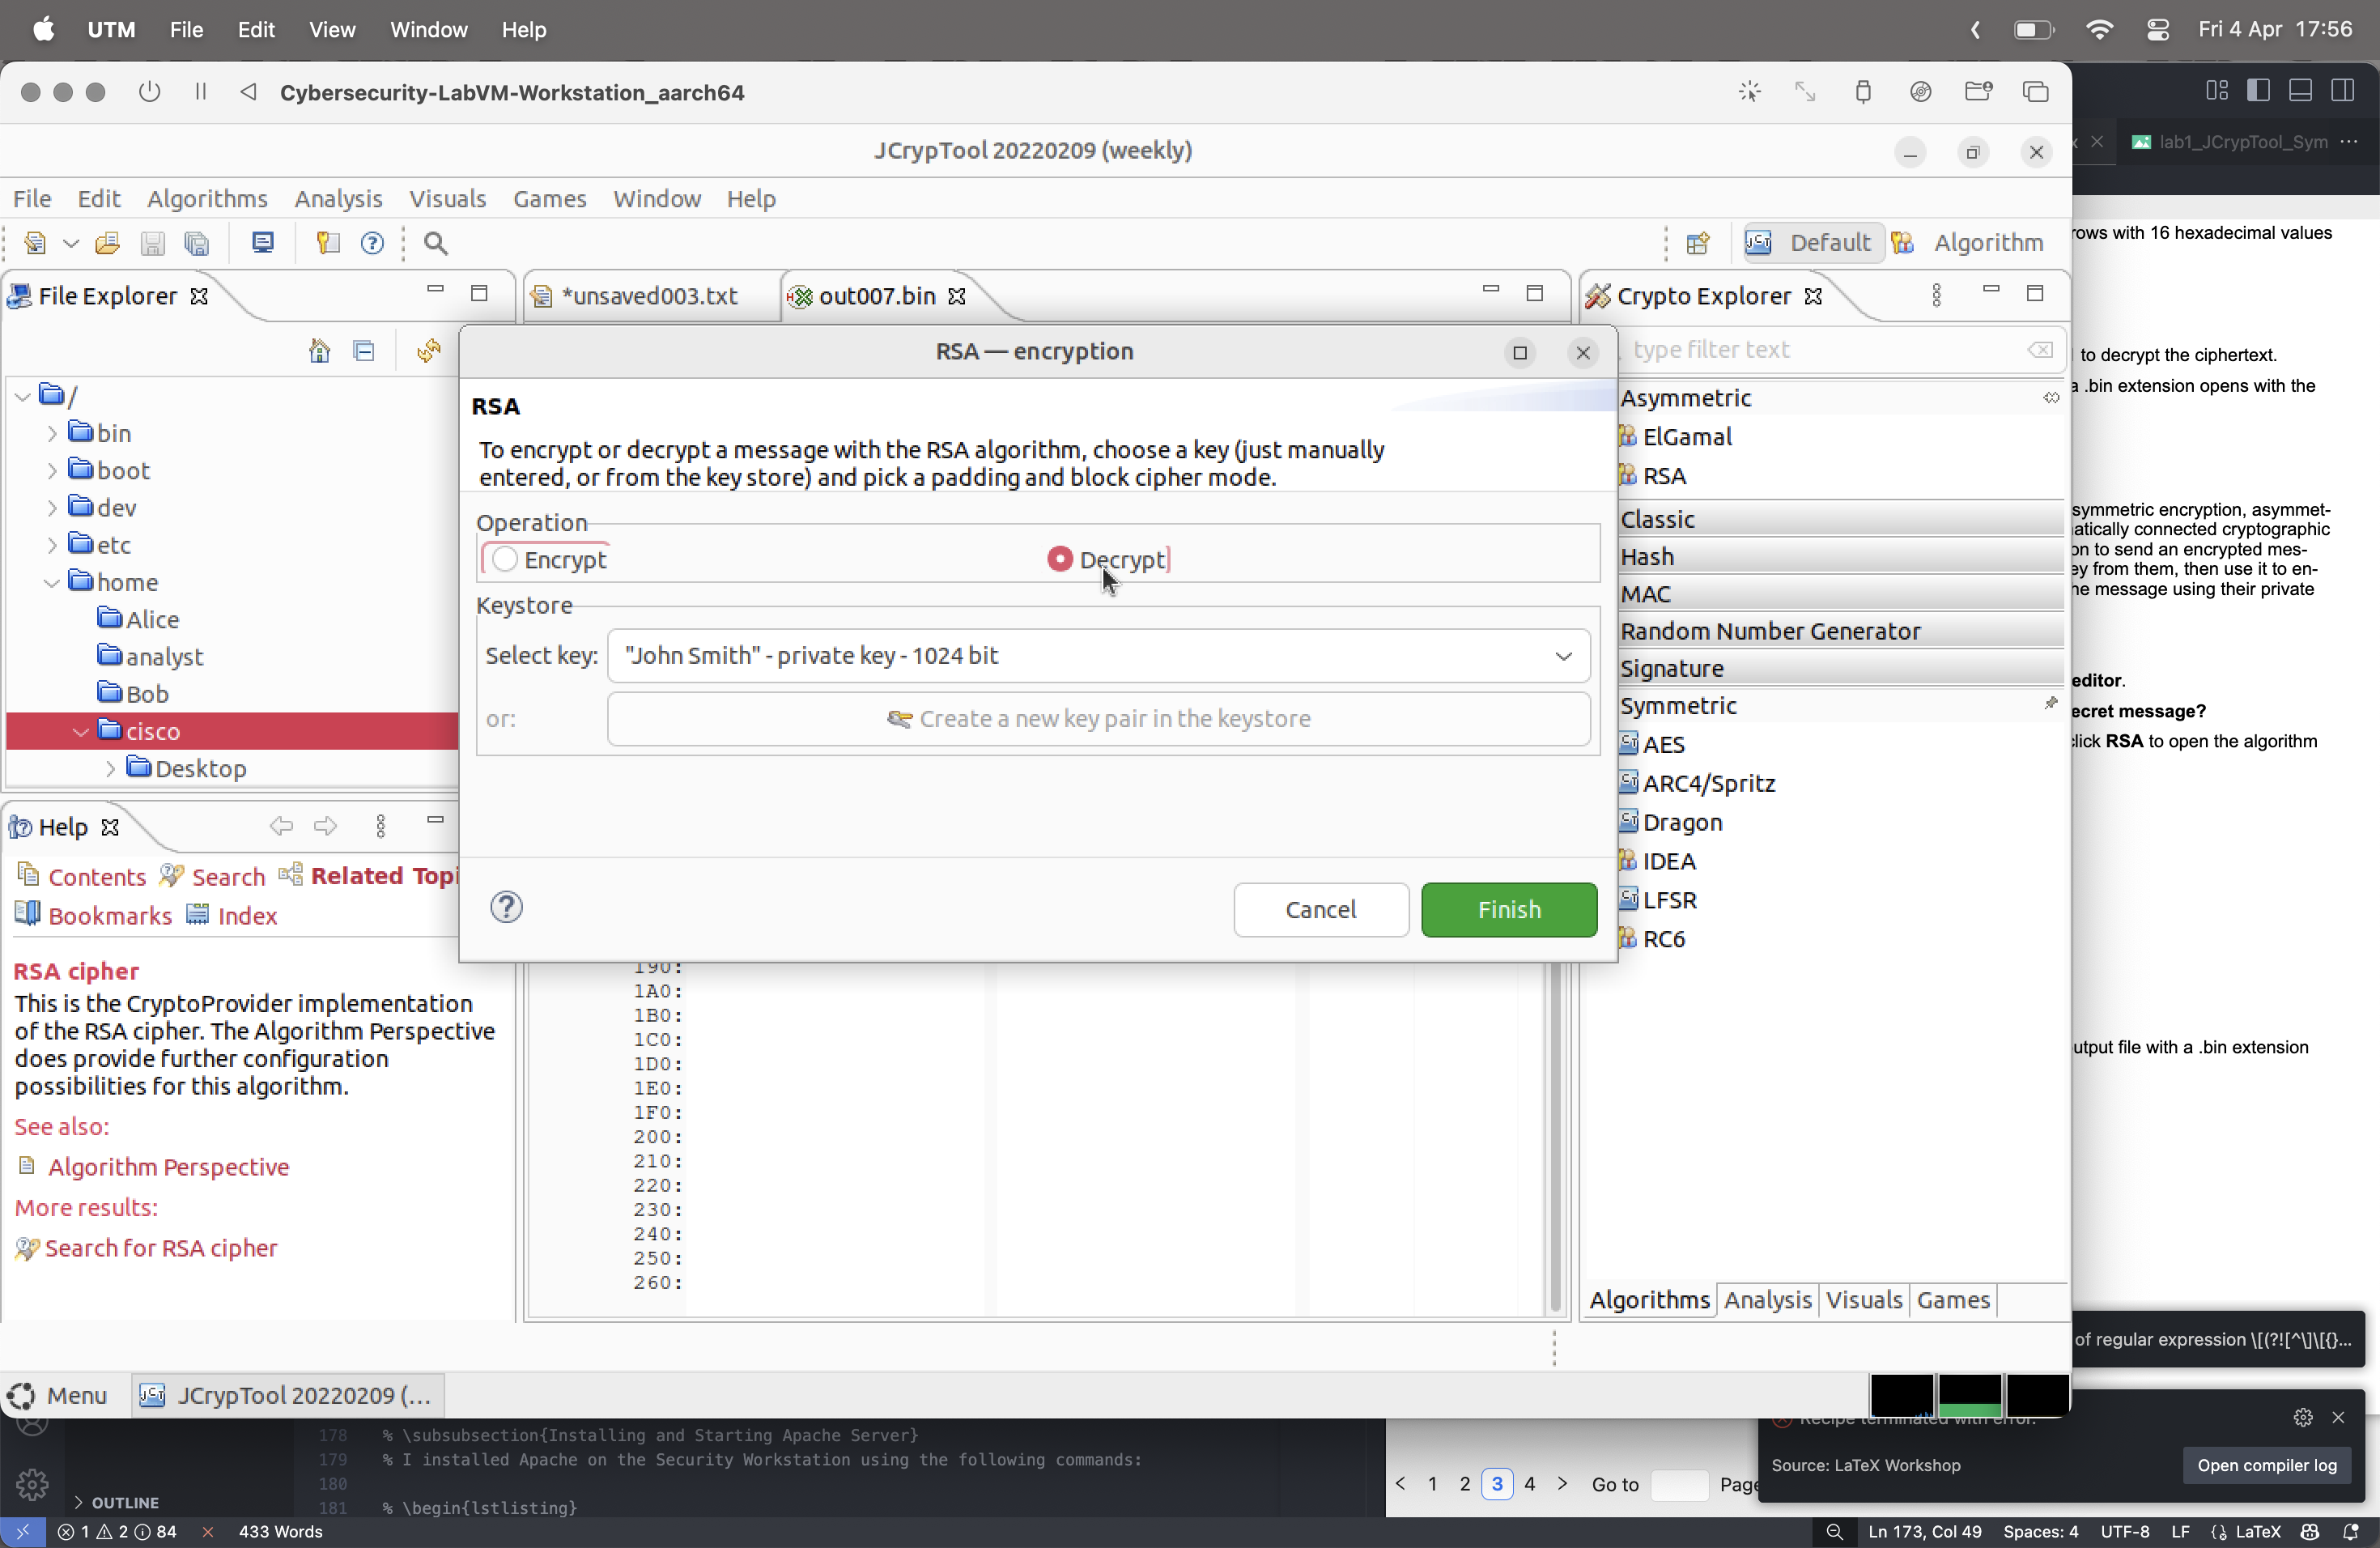
\includegraphics[width=0.8\textwidth]{lab1_JCrypTool_Asymmetric_RSA_decryption.png}
    \caption{JCrypTool Asymmetric RSA decryption}
\end{figure}

and for result I got the same text message "Cryptography is fun. Can you read this secret message?".

\section{Lab 2: Encrypting and Decrypting Data using a Hacker Tool}

\subsection{Create and Encrypt Files}
In this part, I will create a few text files that will be used to created encrypted zip files in the next step.

\subsubsection{Create text files}
I created thee txt files with the same text message "This is a sample text file" in dir Zip-Files.
\begin{figure}[H]
    \centering
    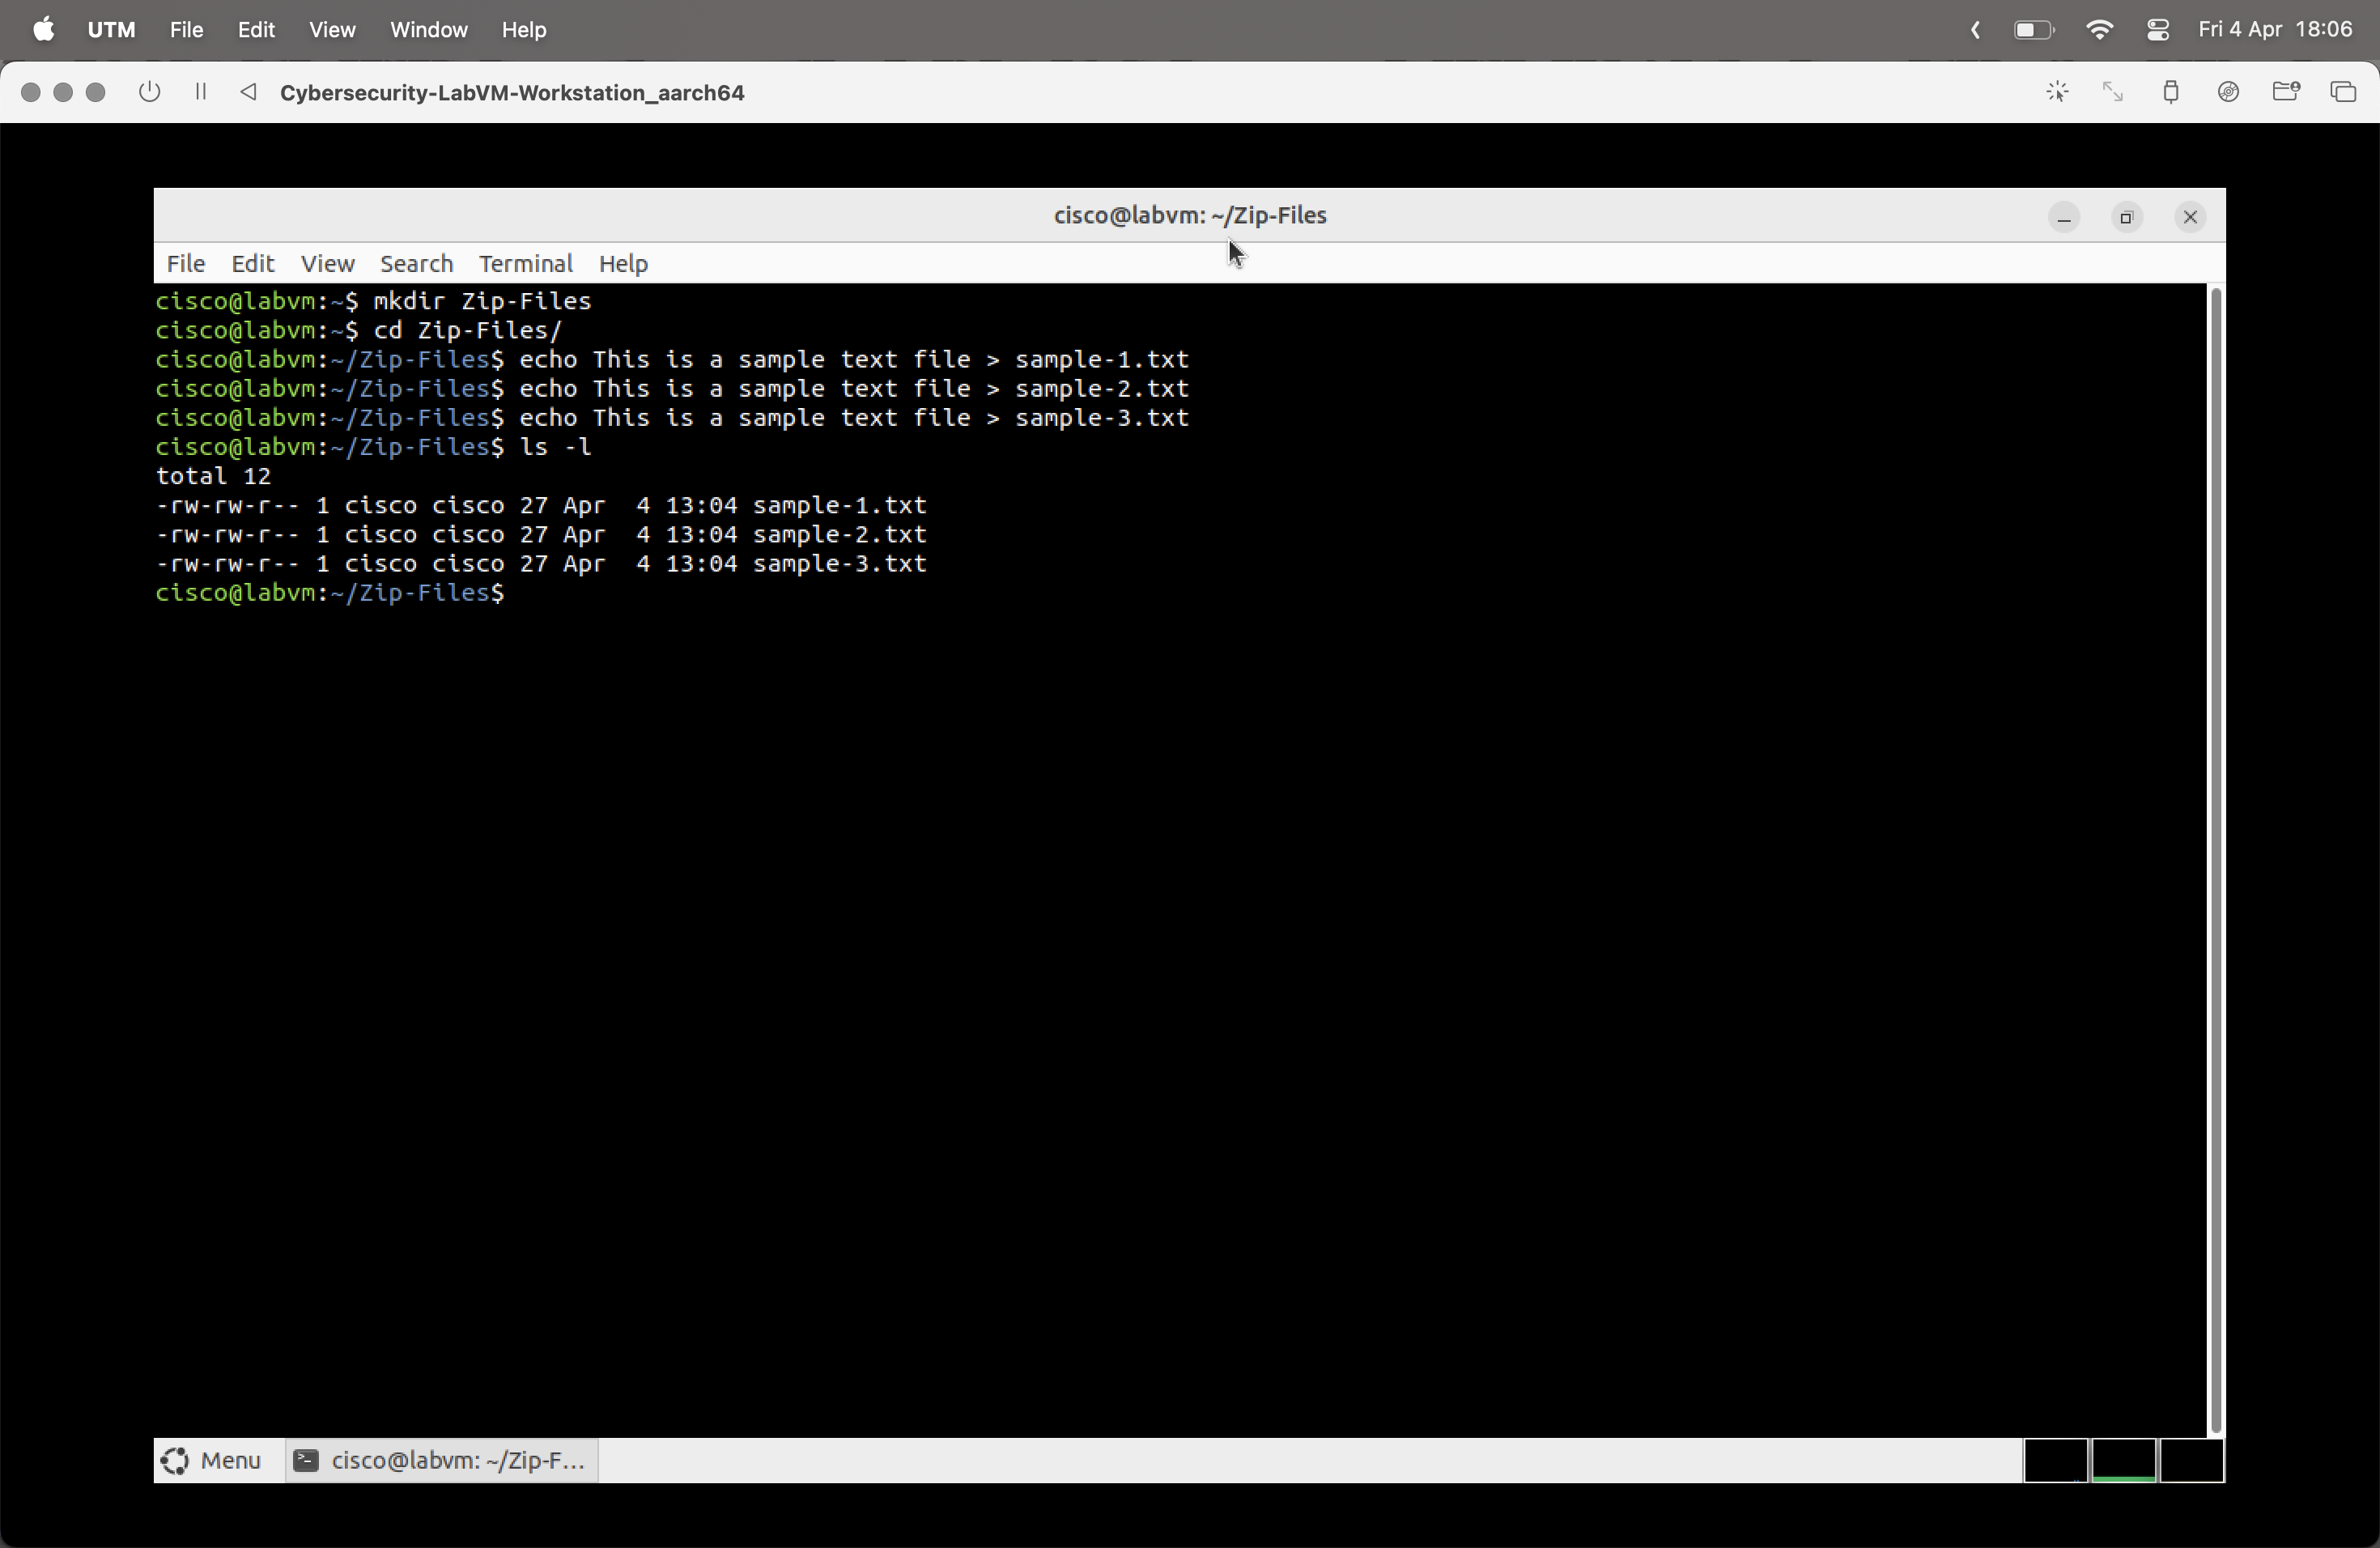
\includegraphics[width=0.8\textwidth]{lab2_new_txt_files.png}
    \caption{Created three txt files}
\end{figure}

\subsubsection{Zip and encrypt the text files.}
There I created 5 zip files with different passwords, I used the same text files for zipping, and command was:
\texttt{zip -e file-N.zip sample-*}

And passwords were:
\begin{itemize}
    \item file-1.zip: B
    \item file-2.zip: R2
    \item file-3.zip: 0B1
    \item file-4.zip: Y0Da
    \item file-5.zip: C-3P0
\end{itemize}

in result I got 5 zip files with different passwords:
\begin{figure}[H]
    \centering
    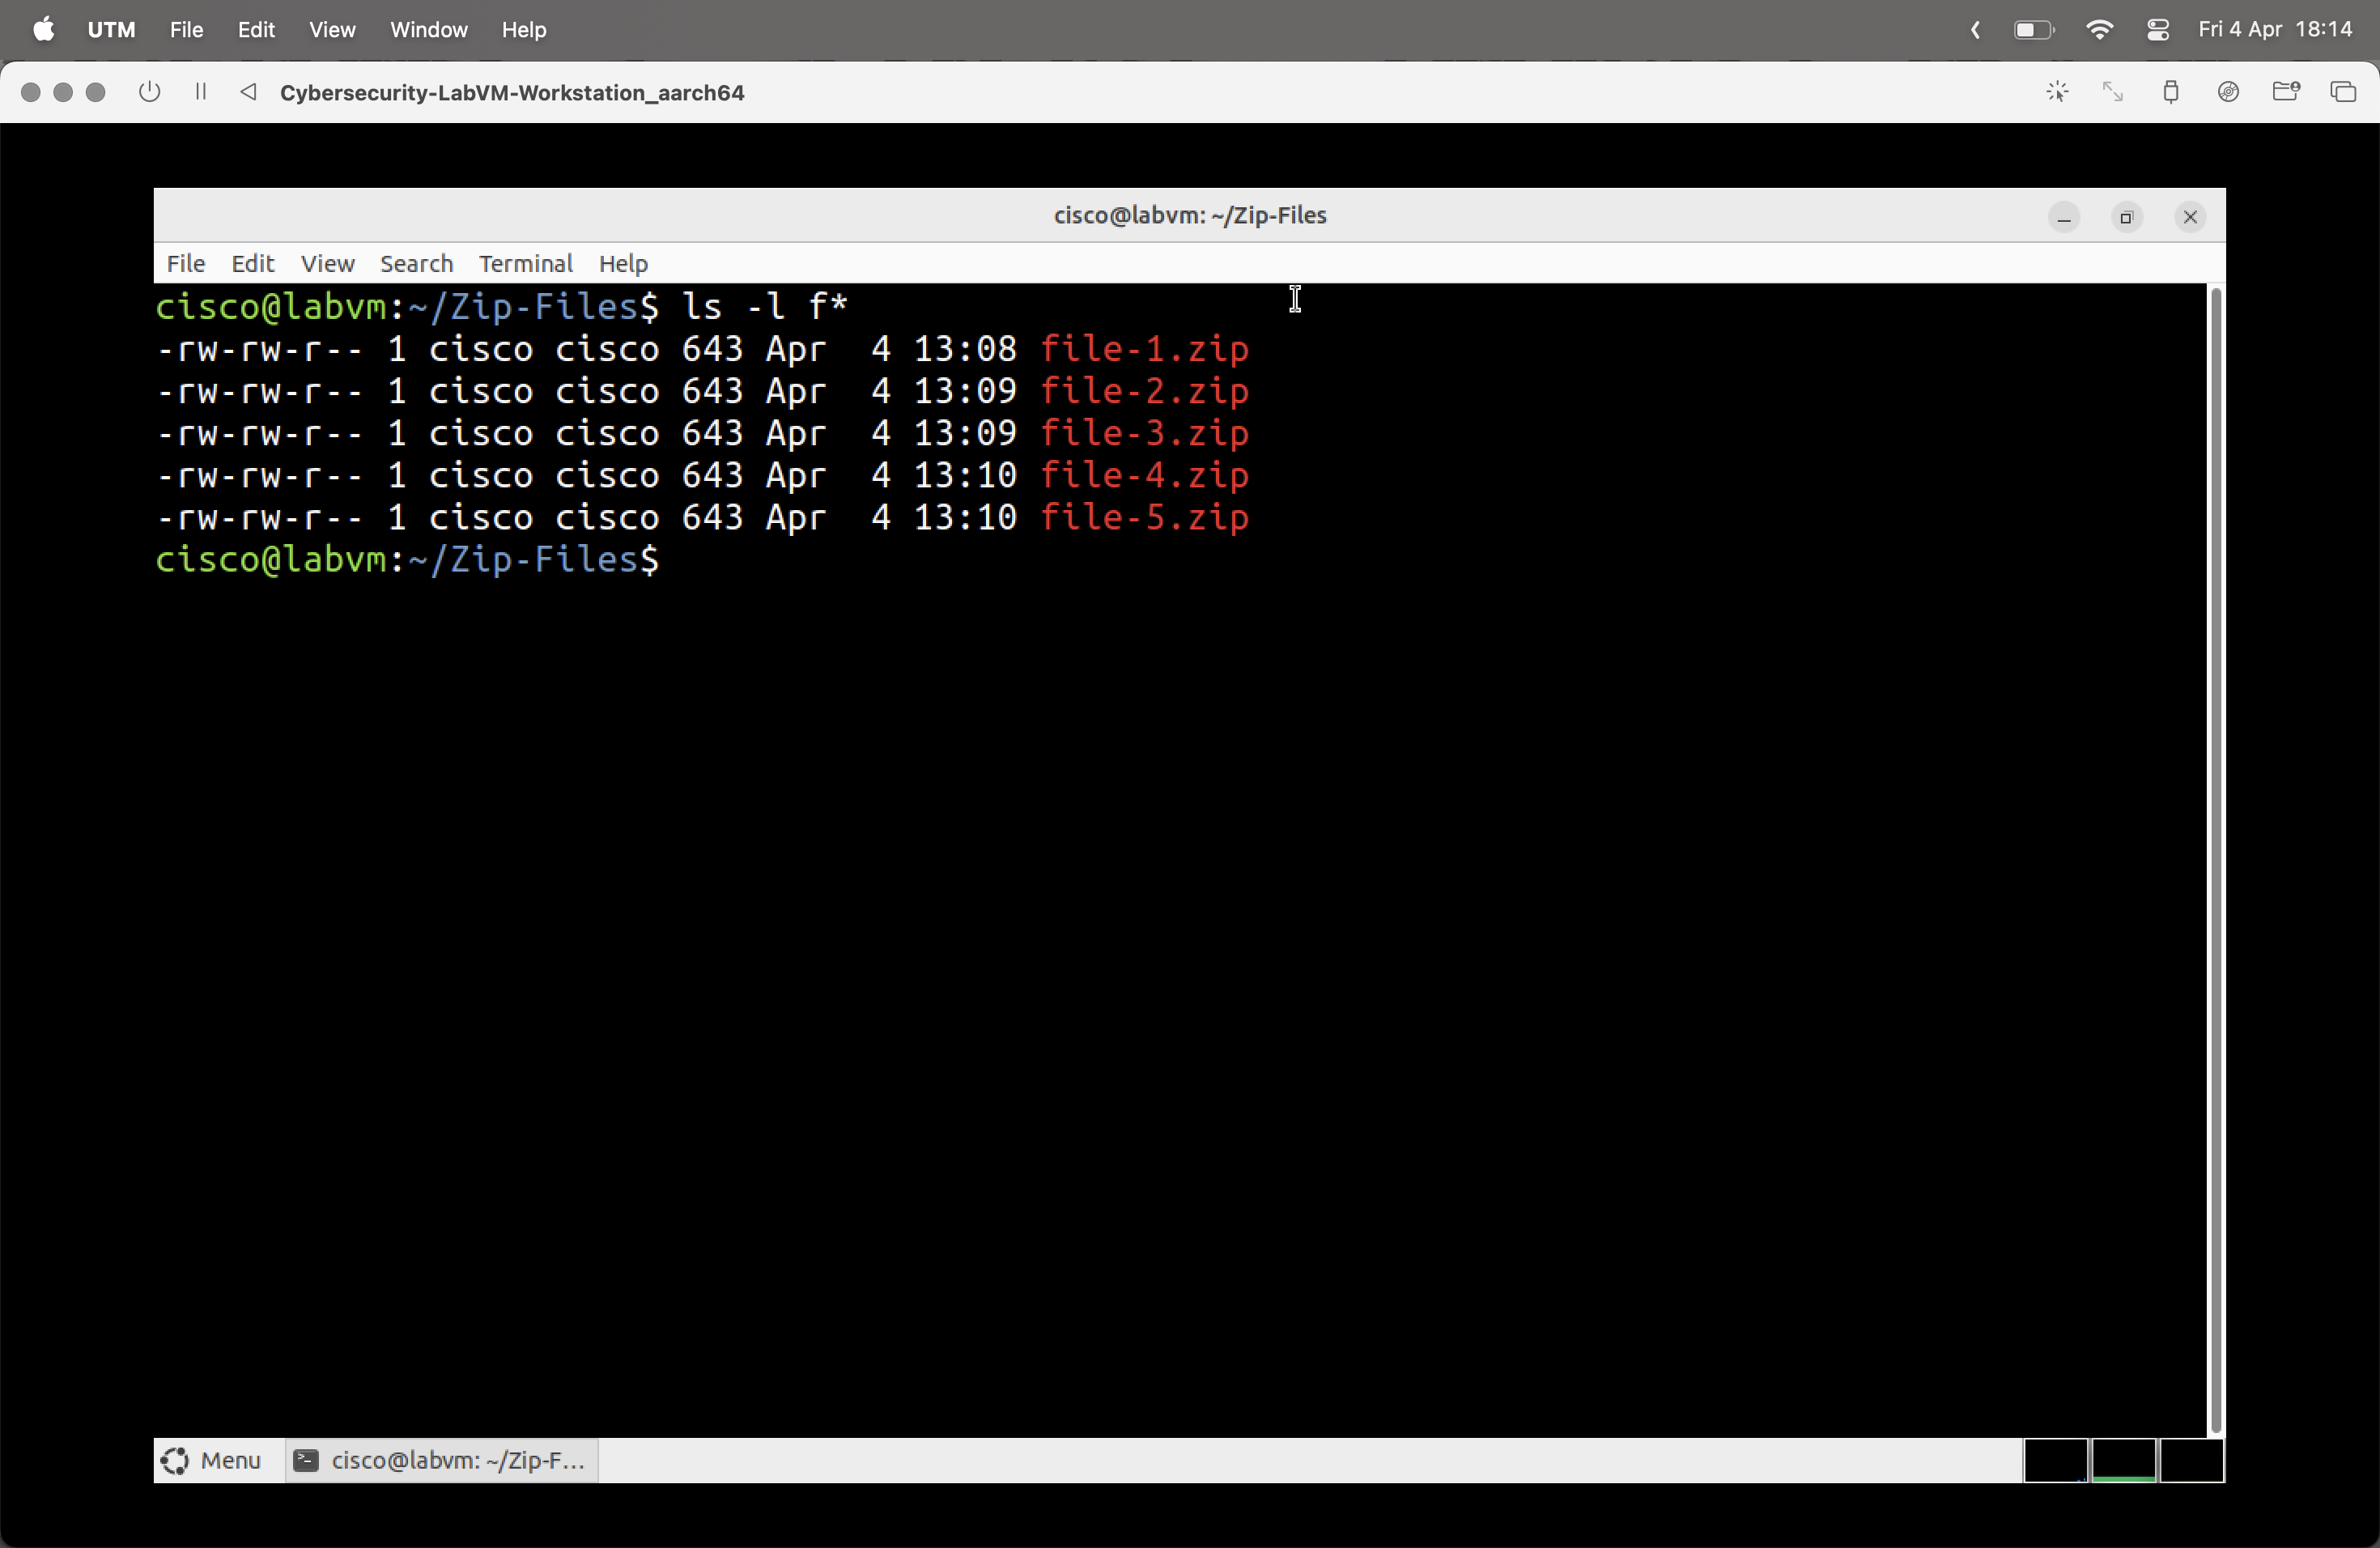
\includegraphics[width=0.8\textwidth]{lab2_zip_files.png}
    \caption{Created 5 zip files}
\end{figure}

\subsection{Recover Encrypted Zip File Passwords}

\subsubsection{Introduction to fcrackzip}
For this part, I check the new terminal command for cracking zip file passwords. The command is fcrackzip.
\begin{figure}[H]
    \centering
    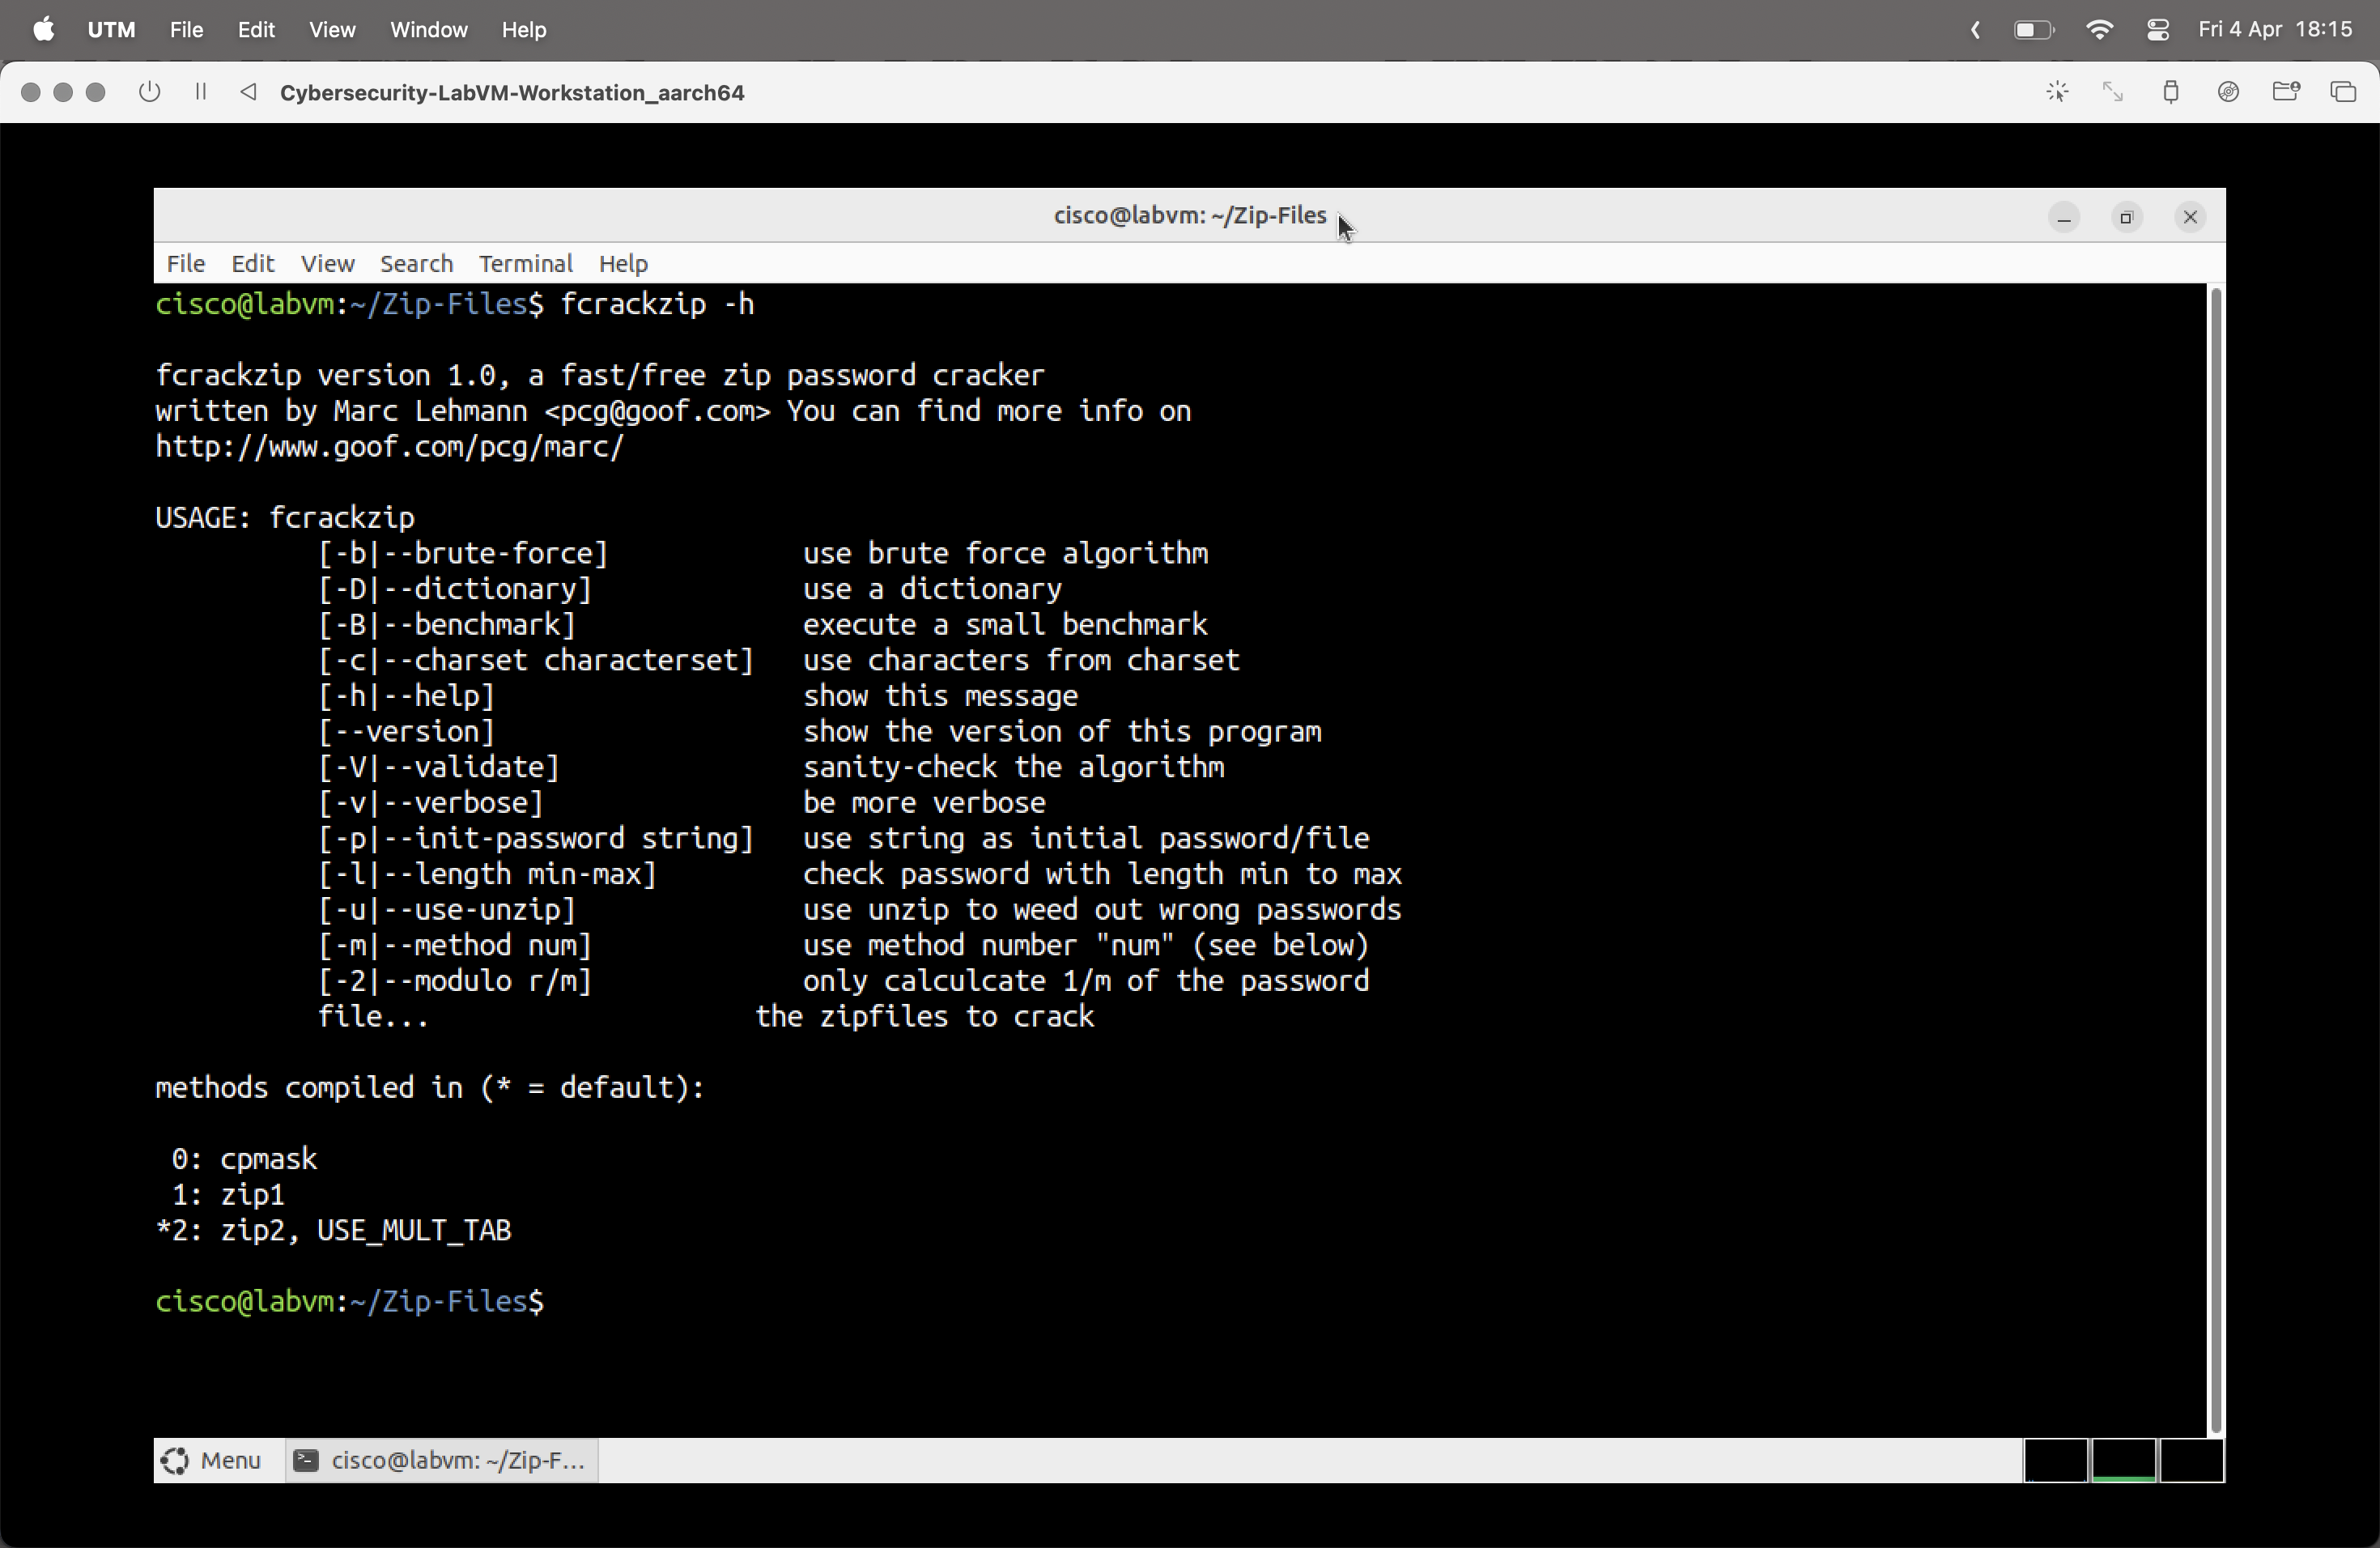
\includegraphics[width=0.8\textwidth]{lab2_fcrackzip.png}
    \caption{fcrackzip command list}
\end{figure}

\subsubsection{Recovering Passwords using fcrackzip}
In this part we will use the fcrackzip command to recover passwords for the zip files we created in the previous parts.
For all files except file-5.zip I used the command(in 5th file we use 1-5 instead of 1-4):
\texttt{fcrackzip -vul 1-4 file-N.zip}

and I got this result for all files(how much time it took to crack the password):
\begin{itemize}
    \item file-1.zip: 0.11 seconds
    \item file-2.zip: 0.6 seconds
    \item file-3.zip: 0.38 seconds
    \item file-4.zip: 1.108 seconds
    \item file-5.zip: 50.194 seconds
\end{itemize}
For calculation I used the Bash-Script:
\begin{lstlisting}[language=bash,caption={bash version}]
    #!/bin/bash

    # Input from command line
    ZIP_FILE=$1
    
    # Start time in milliseconds
    START_MS=$(date +%s%3N)
    
    # Run fcrackzip, adjust the range as needed
    # Here we are using 1-4 for the first four files
    fcrackzip -vul 1-4 "$ZIP_FILE"
    
    # End time in milliseconds
    END_MS=$(date +%s%3N)
    
    # Duration in milliseconds
    DURATION_MS=$((END_MS - START_MS))
    
    # Convert to seconds with milliseconds
    SECONDS=$((DURATION_MS / 1000))
    MILLISECONDS=$((DURATION_MS % 1000))
    
    echo "Time taken: ${SECONDS}.${MILLISECONDS} seconds"
\end{lstlisting}

\begin{figure}[H]
    \centering
    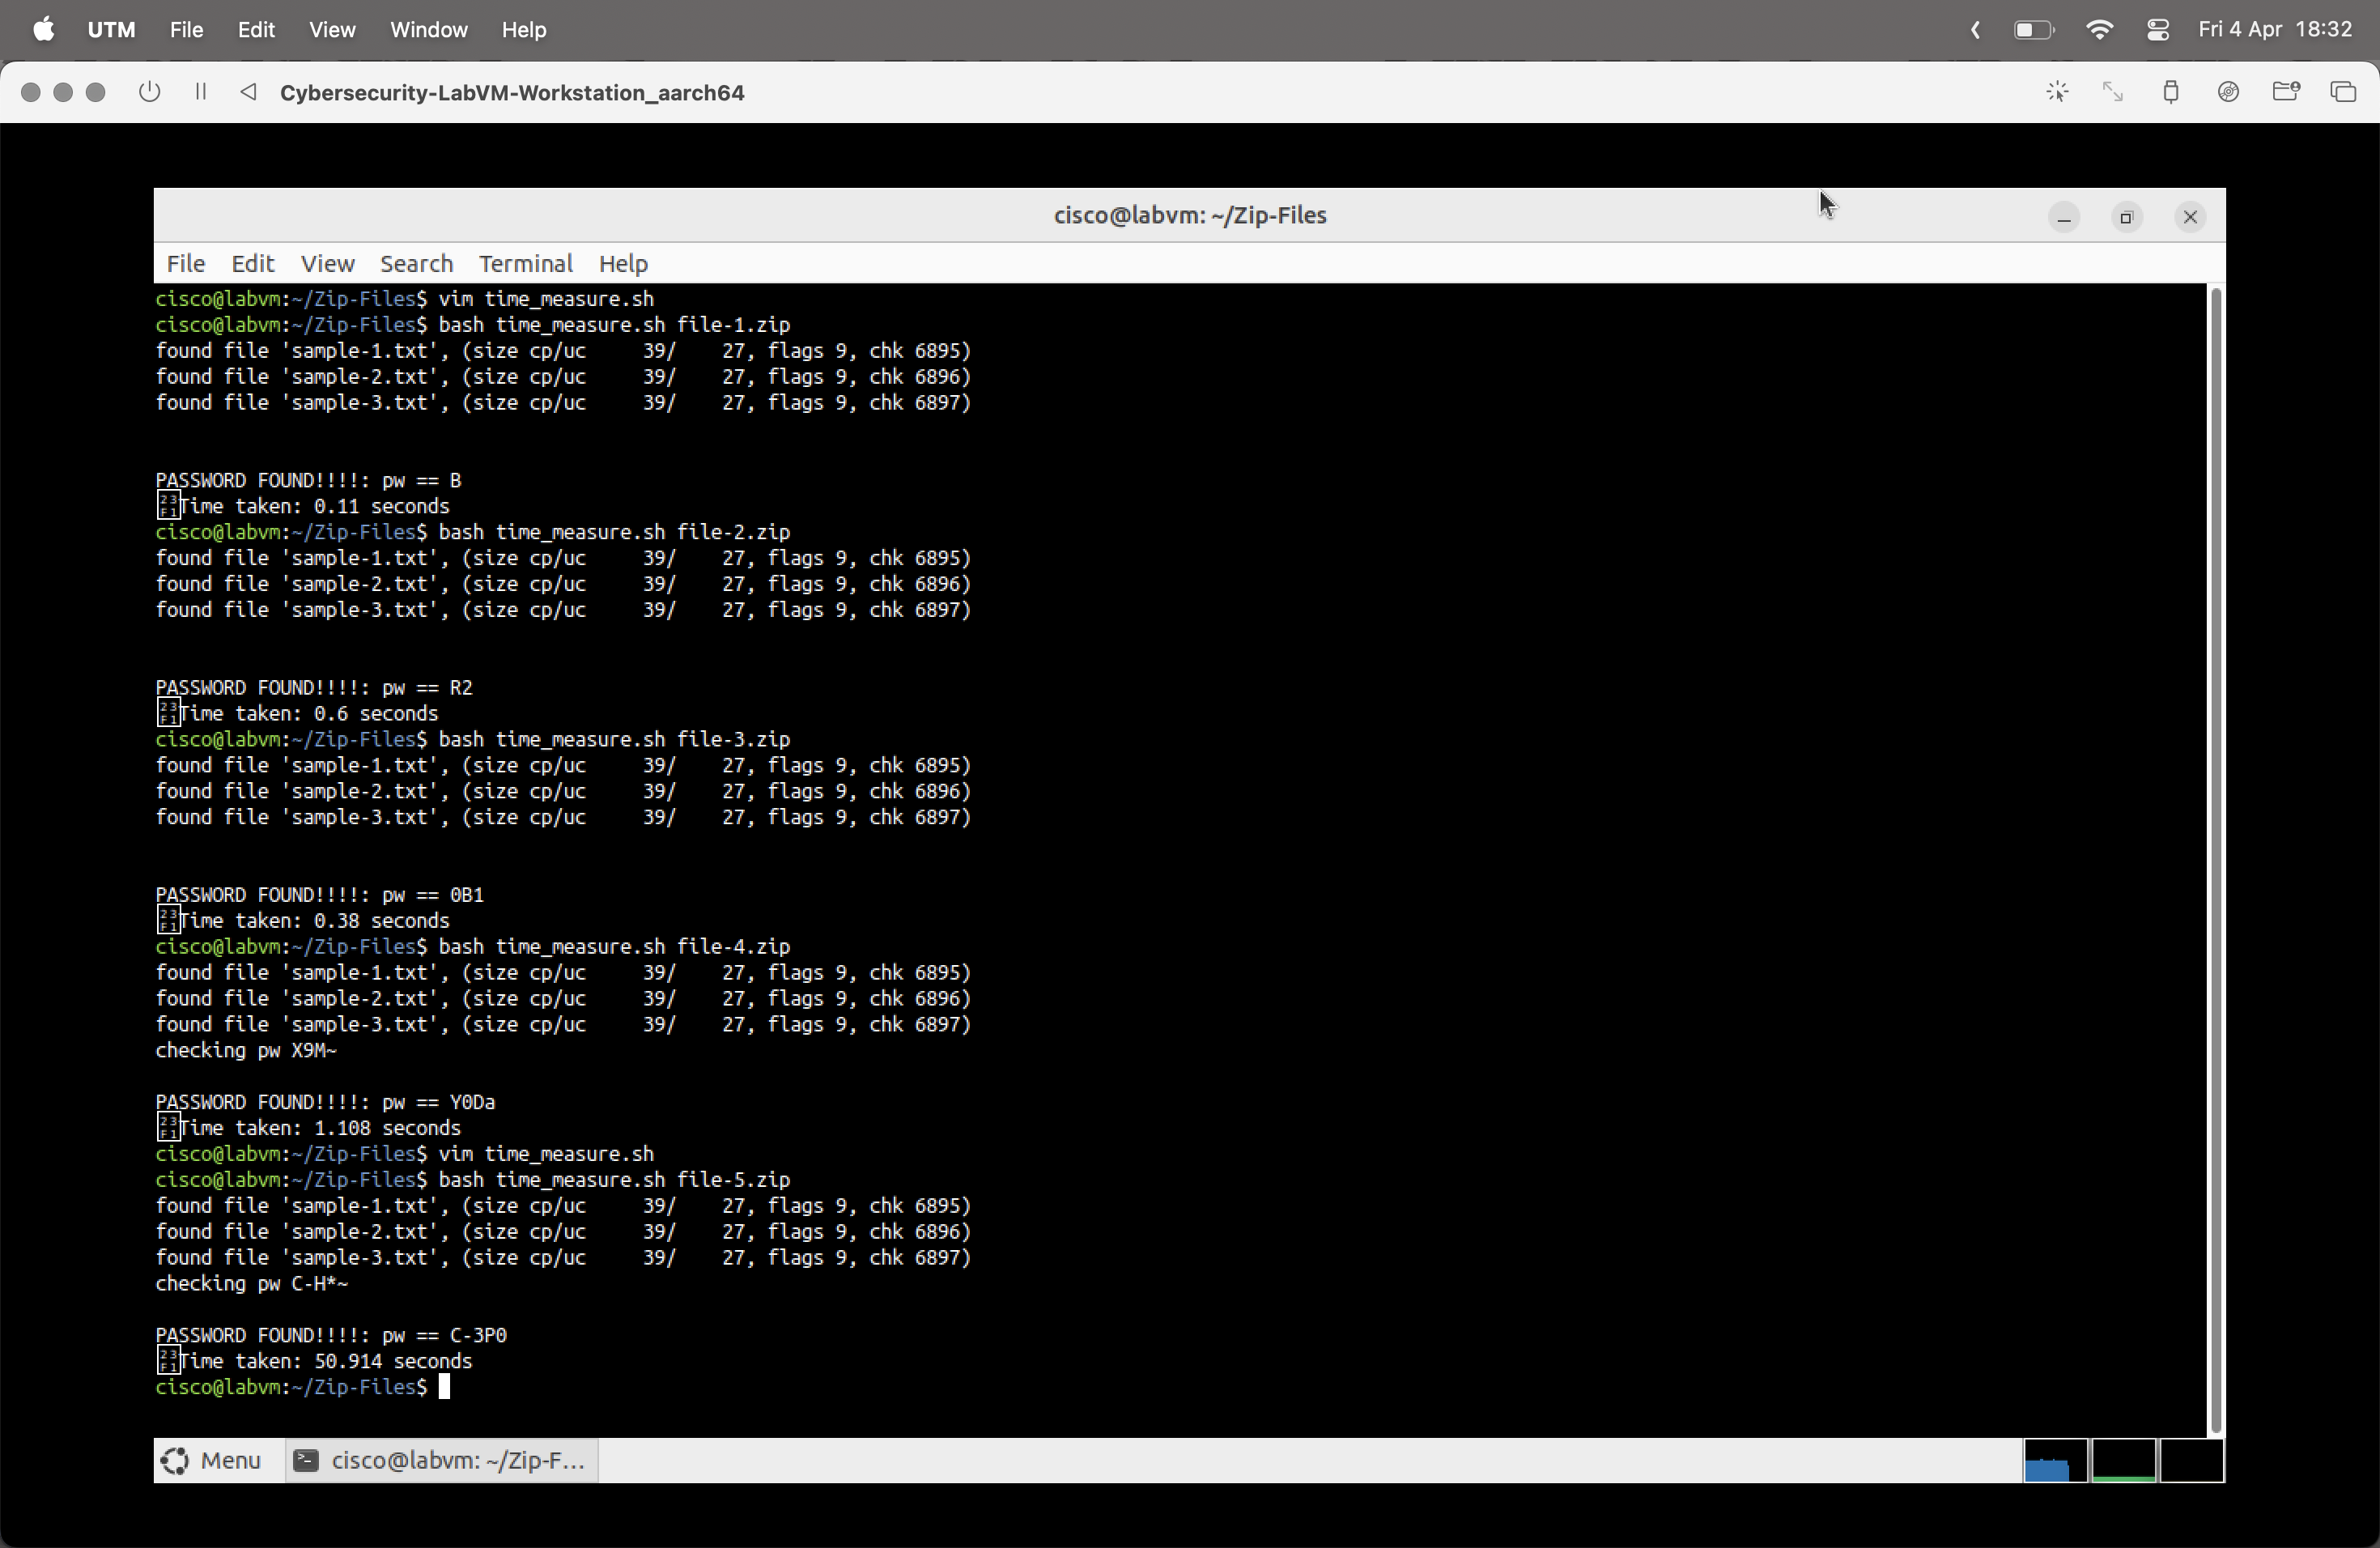
\includegraphics[width=0.8\textwidth]{lab2_cracking_result.png}
    \caption{Result of cracking zip files}
\end{figure}

For interest I also tried to crack the password with 6 Characters(how said in lab), and for that I created file-6.zip with password JarJar. First I thought that it will take 30-40 minutes approximately, but it took 5315,617 seconds, which is about 1.5 hours.
The last question was about what I recommend a password needs to be for it to be secure, and I think that password should be at least 8 characters long and contain a mix of characters, including uppercase and lowercase letters, numbers, and special characters. This makes it more difficult for attackers to guess or crack the password using brute force methods.

\end{document}